\documentclass[10pt,a4paper,twocolumn]{article}
\usepackage[utf8]{inputenc}
\usepackage[english]{babel}
\usepackage{amsmath}
\usepackage{amsfonts}
\usepackage{amssymb}
\usepackage{makeidx}
\usepackage{natbib}
\usepackage{graphicx}
\usepackage{hyperref}
\usepackage{lscape}
\usepackage{appendix}
\usepackage{midpage}
\usepackage{gensymb}
\usepackage{geometry}
\usepackage{color}
\geometry{top=1cm, bottom=2cm, left=1.5cm, right=1.5cm}
\setlength{\columnsep}{1cm}


\author{Matteo Malucchi \hspace{2.5cm}  Lorenzo Punzi}
\title{\textbf{POSITRON ANNIHILATION}}
\begin{document}
\date{April 2022}

\twocolumn[
  \begin{@twocolumnfalse}
  \maketitle
    \begin{abstract}
      \noindent The mass of the electron has been measured by measuring the energy of photons emitted in pair annihilation between electrons in various mediums and positrons generated by a radioactive Na source. The measure yielded the result $m_e=510.1 \pm 0.5 \text{ (sys)} \pm 0.3 \text{ (stat) KeV}$. Subsequently tests were made to observe triple $\gamma$ pair annihilation processes and measure their rate, which was then compared to the double $\gamma$ rate previously found in order to obtain an estimate of the fine structure constant $\alpha_{em}$. This measure yielded the result $\alpha_{em}=  0.2990 \pm   0.0001$, with an unknown systematic error much bigger than the statistical one reported. Finally evidence of a state with not null mean life was found( $\tau=2.6 \pm 0.2 \; \text{ns}$). 
      \bigskip
      \bigskip
      \bigskip
     
    \end{abstract}
  \end{@twocolumnfalse}
]

\section{INTRODUCTION}

The $^{22}$Na atom decays emitting a low energy positron (544 KeV), which quickly annihilates with an electron in matter to produce 2$\gamma$ (or rarely 3$\gamma$). Under the reasonable assumption that the $e^+$ loses almost all of its kinetic energy $T$ before annihilating, the resulting 2 photons have total energy $k_1+k_2 \simeq m_{e^-}+m_{e^+}=2m_e$. The equation is only approximately valid because in reality neither the positron nor the electron are perfectly at rest when they annihilate, but their kinetic energies are much smaller than their mass of 511 KeV (typically on the scale of eV, since the positron usually thermalizes with the material). Also, if the above approximation holds true, then the two photons should both have the same energy ($m_e$) (apart from $T/m_e$  corrections), because in such case the lab frame is essentially the rest frame, in which two body decays are monochromatic and thus if the two products are identical so are their energies. Measuring said energy is therefore a way of measuring the mass of the electron.

Furthermore, by measuring the rate of the rarer 3$\gamma$ decay and its relative frequency compared to the 2$\gamma$ decay, it is possible to evaluate the fine structure constant $\alpha_{em}=e^2/\hbar c$.

Finally the presence of the higher energy $^{22}$Ne* photon (see \figurename~\ref{fig:22na}) and the possibility of recording the relative times between the detection of these photons allow for the search of possible states with non null mean lifetimes. 

\begin{figure}[h!]
\centering
\includegraphics[scale=0.55]{22na_decay.png} 
\caption{$^{22}$Na decay scheme.}
\label{fig:22na}
\end{figure}

\section{INITIAL SETUP AND CALIBRATION }


In order to observe double $\gamma$ decays and measure $m_e$ a calibration of the detector, made up of NaI crystals and their pmts, is needed. For the calibration radioactive test sources of $^{60}$Co and $^{137}$Cs were used (see \figurename~\ref{fig:60co}, \figurename~\ref{fig:137cs}). 

\begin{figure}[h!]
\centering
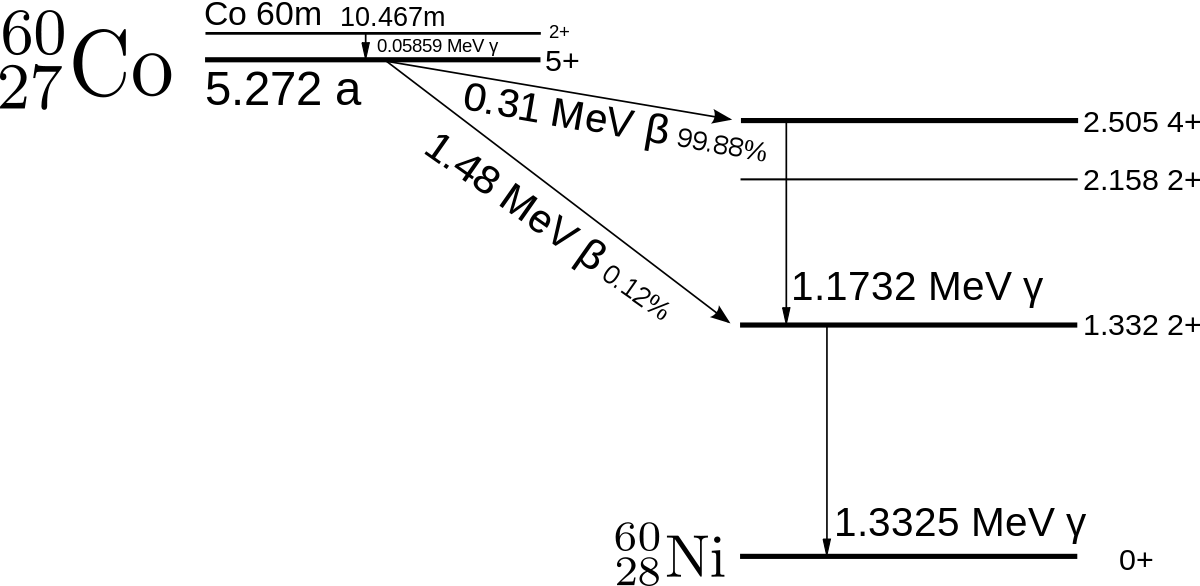
\includegraphics[scale=0.15]{co.png} 
\caption{$^{60}$Co dacay scheme.}
\label{fig:60co}
\end{figure}

\begin{figure}[h!]
\centering
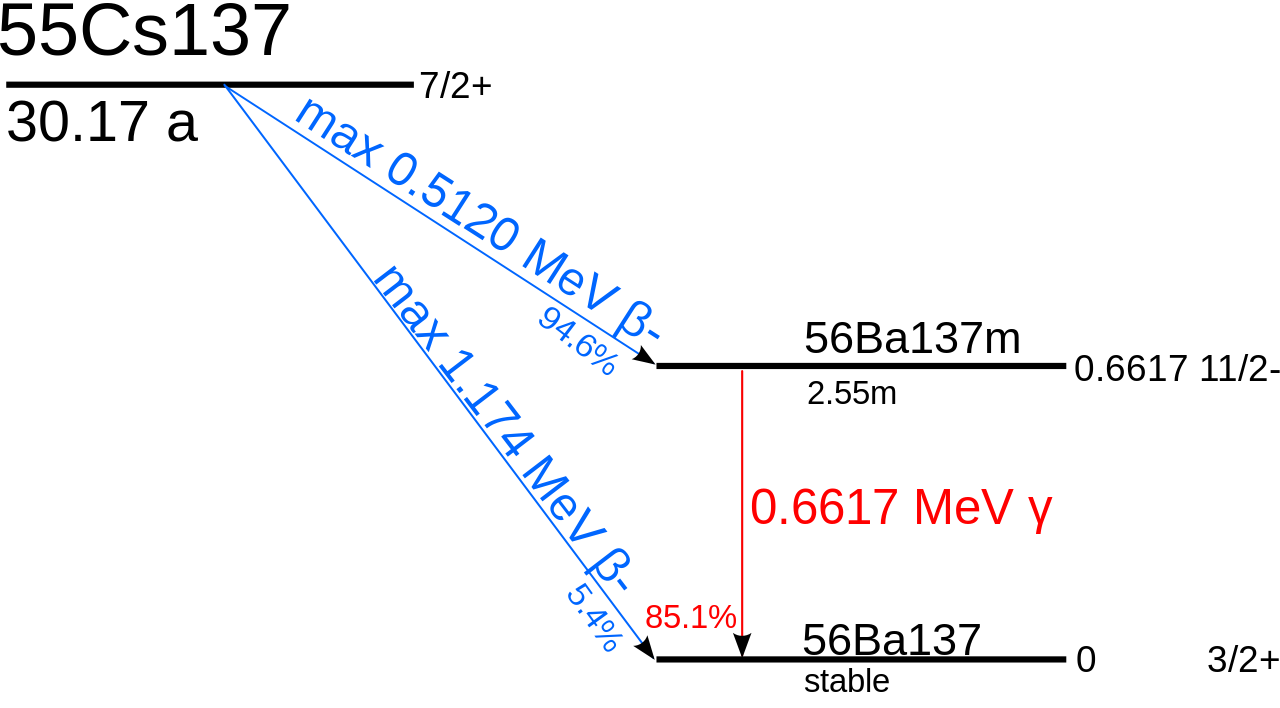
\includegraphics[scale=0.15]{cs.png} 
\caption{$^{137}$Cs decay scheme.}
\label{fig:137cs}
\end{figure}

The waveforms emitted by the pmts are digitalized with a 14 bit ADC unit \footnote{A list of the specific models used can be found in Appendix \ref{appendix:strumentation}} @250 MHz (see \figurename~\ref{fig:wave}) and the entirety of the acquisition lasts $4.12 \mu s$ \footnote{Each waveform contains 1030 samples, each representing a 4 $ns$ interval}. 

\begin{figure}[h!]
\centering
\caption{Example of a digitalized waveform. [07/04/22]}
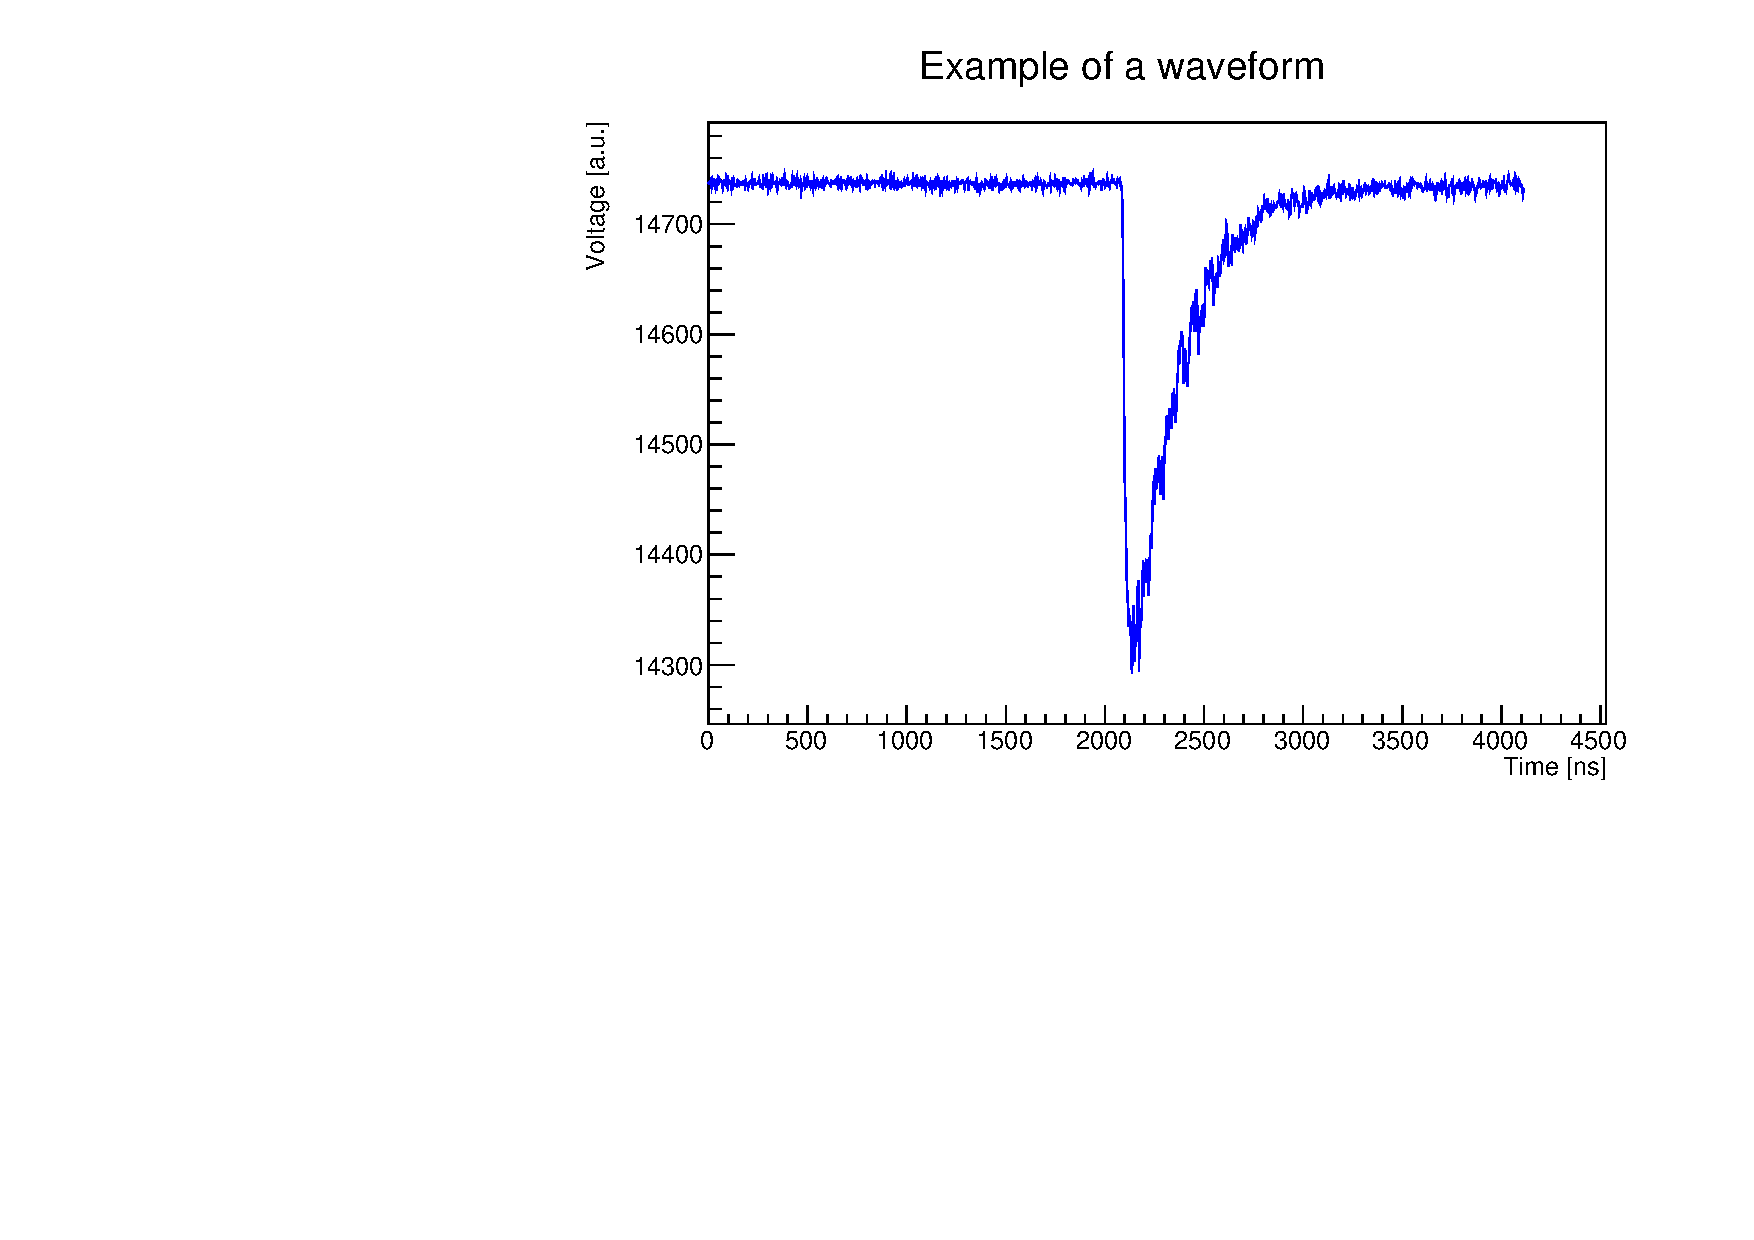
\includegraphics[scale=0.4]{Lab4/Positronio/waveform.pdf} 
\label{fig:wave}
\end{figure}

Such unit only accepts pulses no more than 2 V peak-to-peak high, so in every instance over the course of the data collection the power supply voltages of the pmts were regulated so as to only emit pulses in such range. The voltages for the 3 pmts available were ultimately set to 

\begin{equation}
    V^{PS}_{1}\simeq 690 \text{ V}\quad , \quad V^{PS}_{2} \simeq 851 \text{ V} \quad , \quad V^{PS}_{3} \simeq 761 \text{ V}
\end{equation}  

These voltages were chosen since they were the highest possible that prevented 2 V peak-to-peak events from occurring. Furthermore, they are reported with $\simeq$ because they tended to oscillate by 1-2 V day by day, but always around the values reported above.

When an incoming photon interacts with a NaI crystal and the latter scintillates, some of the photons released by the crystal don't make it to the photocathode. Also, the pmt has a certain variability in amplification factor; it has a finite resolution. As a first approximation, it can be assumed that the average charge of the photopeak produced by an incoming photon of energy E is a linear function of E. Thus, by measuring and fitting with a linear function the average charge of the photopeaks of photons emitted by sources of known energy, it is possible to calibrate the apparatus and thus obtain the energy released as a function of the measured charge. The same reasoning can be applied to the amplitude of the signal generated by the pmt, hence  two distinct calibrations for each pmt have been made. The two algorithms for the computation of charge and amplitude are explained in \appendixname~\ref{appendix:c_a_algorithm}.


The charge and amplitude spectra of $^{60}$Co, $^{137}$Cs and $^{22}$Na on the pmt1 are shown in \figurename~\ref{fig:chargespectra} and \figurename~\ref{fig:amplitudespectra}. In these spectra for each photon energy the photoelectric photopeak, the compton plateau and sometimes the backscatter peaks can be observed. Of course in the case of $^{22}$Na, the photon is one of the two produced in the annihilation of the positron. These spectra were taken by triggering on the single pmt using the ADC's internal trigger, setting the threshold to 100 (which is equivalent to about 12 mV) so as to not cut the important features of the spectrum.

The resolution of the detectors is about 3\% on the charge spectrum and about 6\% on the amplitude spectra. This evidently means that the amplitude of the waveform is a less precise estimator of the energy released in the event than charge. This difference can be observed in the spectra, where in amplitude peaks are more merged together compared to charge. 

 \begin{figure}[h!]
\centering
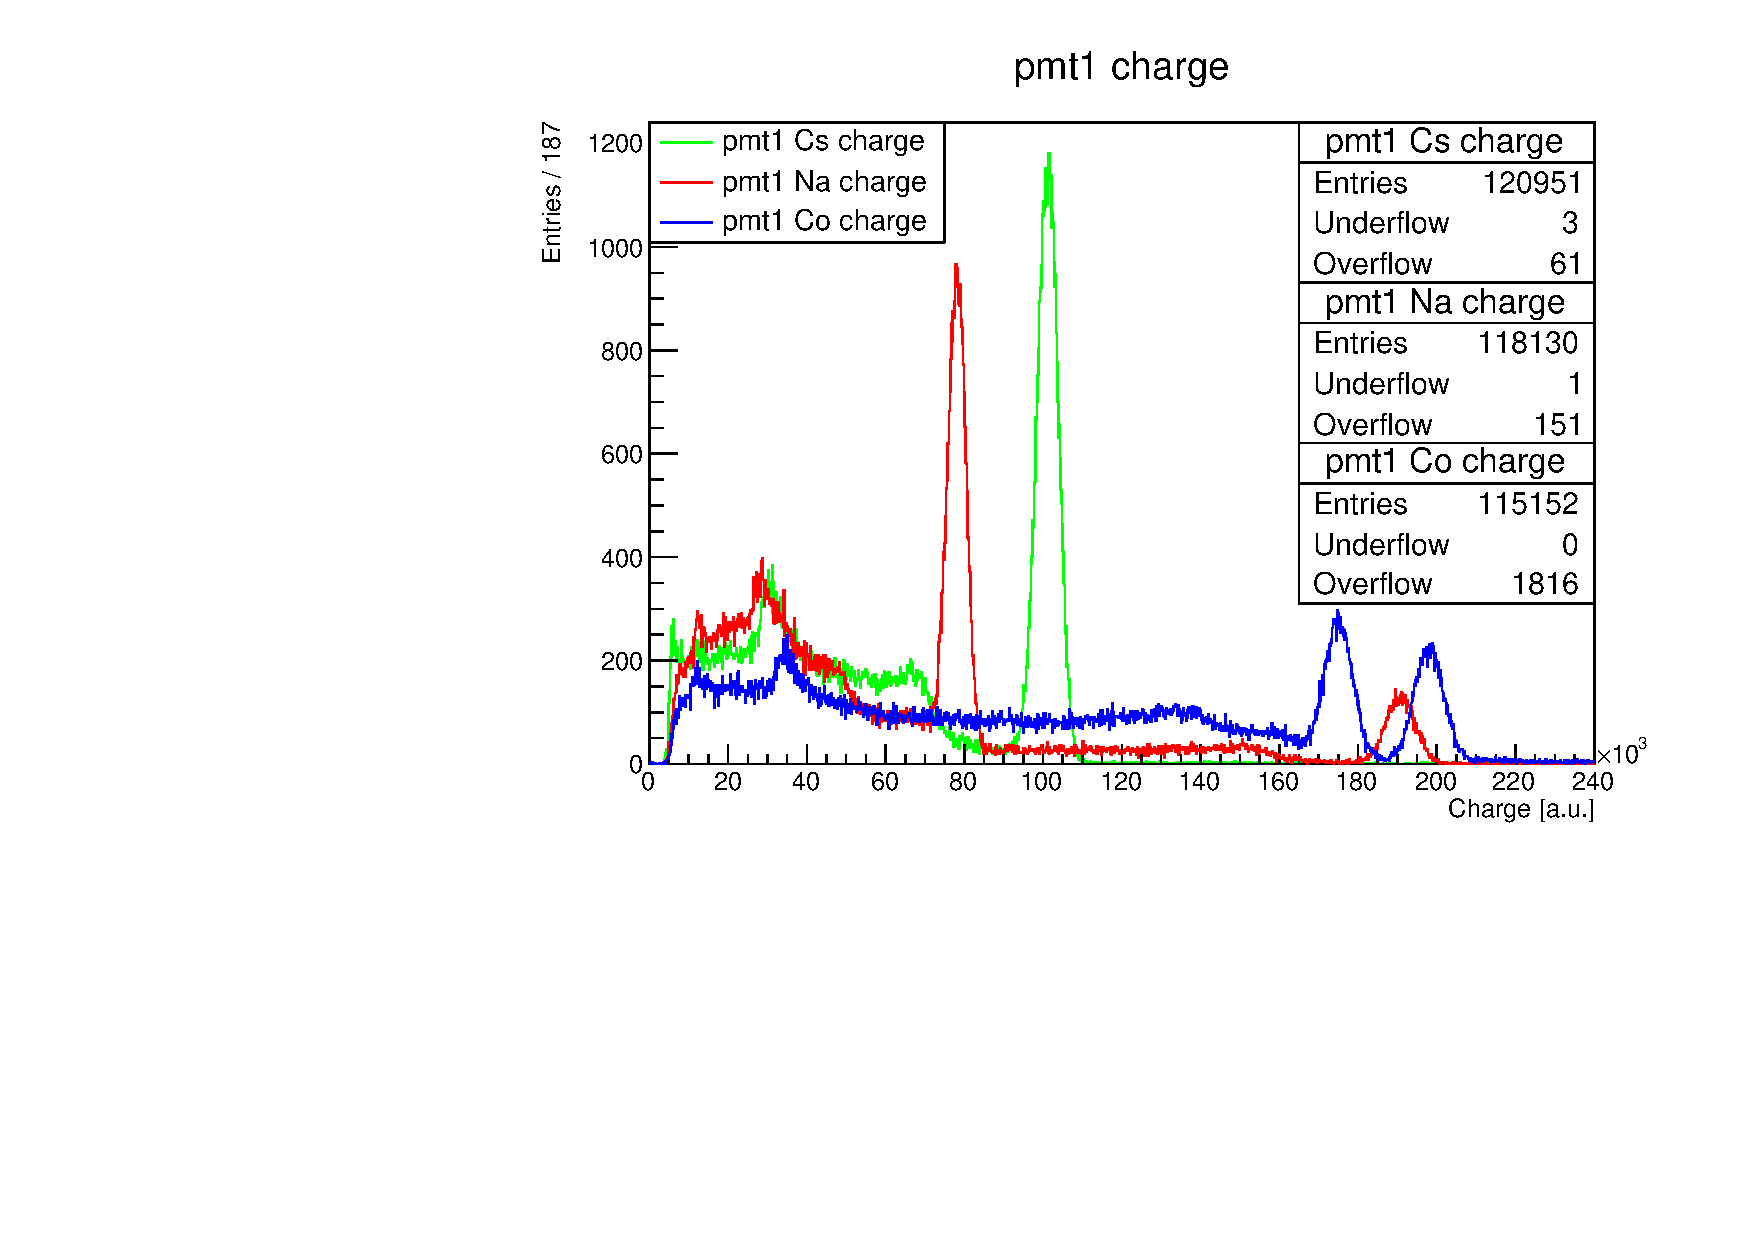
\includegraphics[scale=0.4]{Lab4/Positronio/pmt1_charge.pdf} 
\caption{$^{60}$Co, $^{137}$Cs and $^{22}$Na charge spectra.[Co: 03/03/22][Cs: 03/03/22][Na: 15/03/22]}
\label{fig:chargespectra}
\end{figure}

 \begin{figure}[h!]
\centering
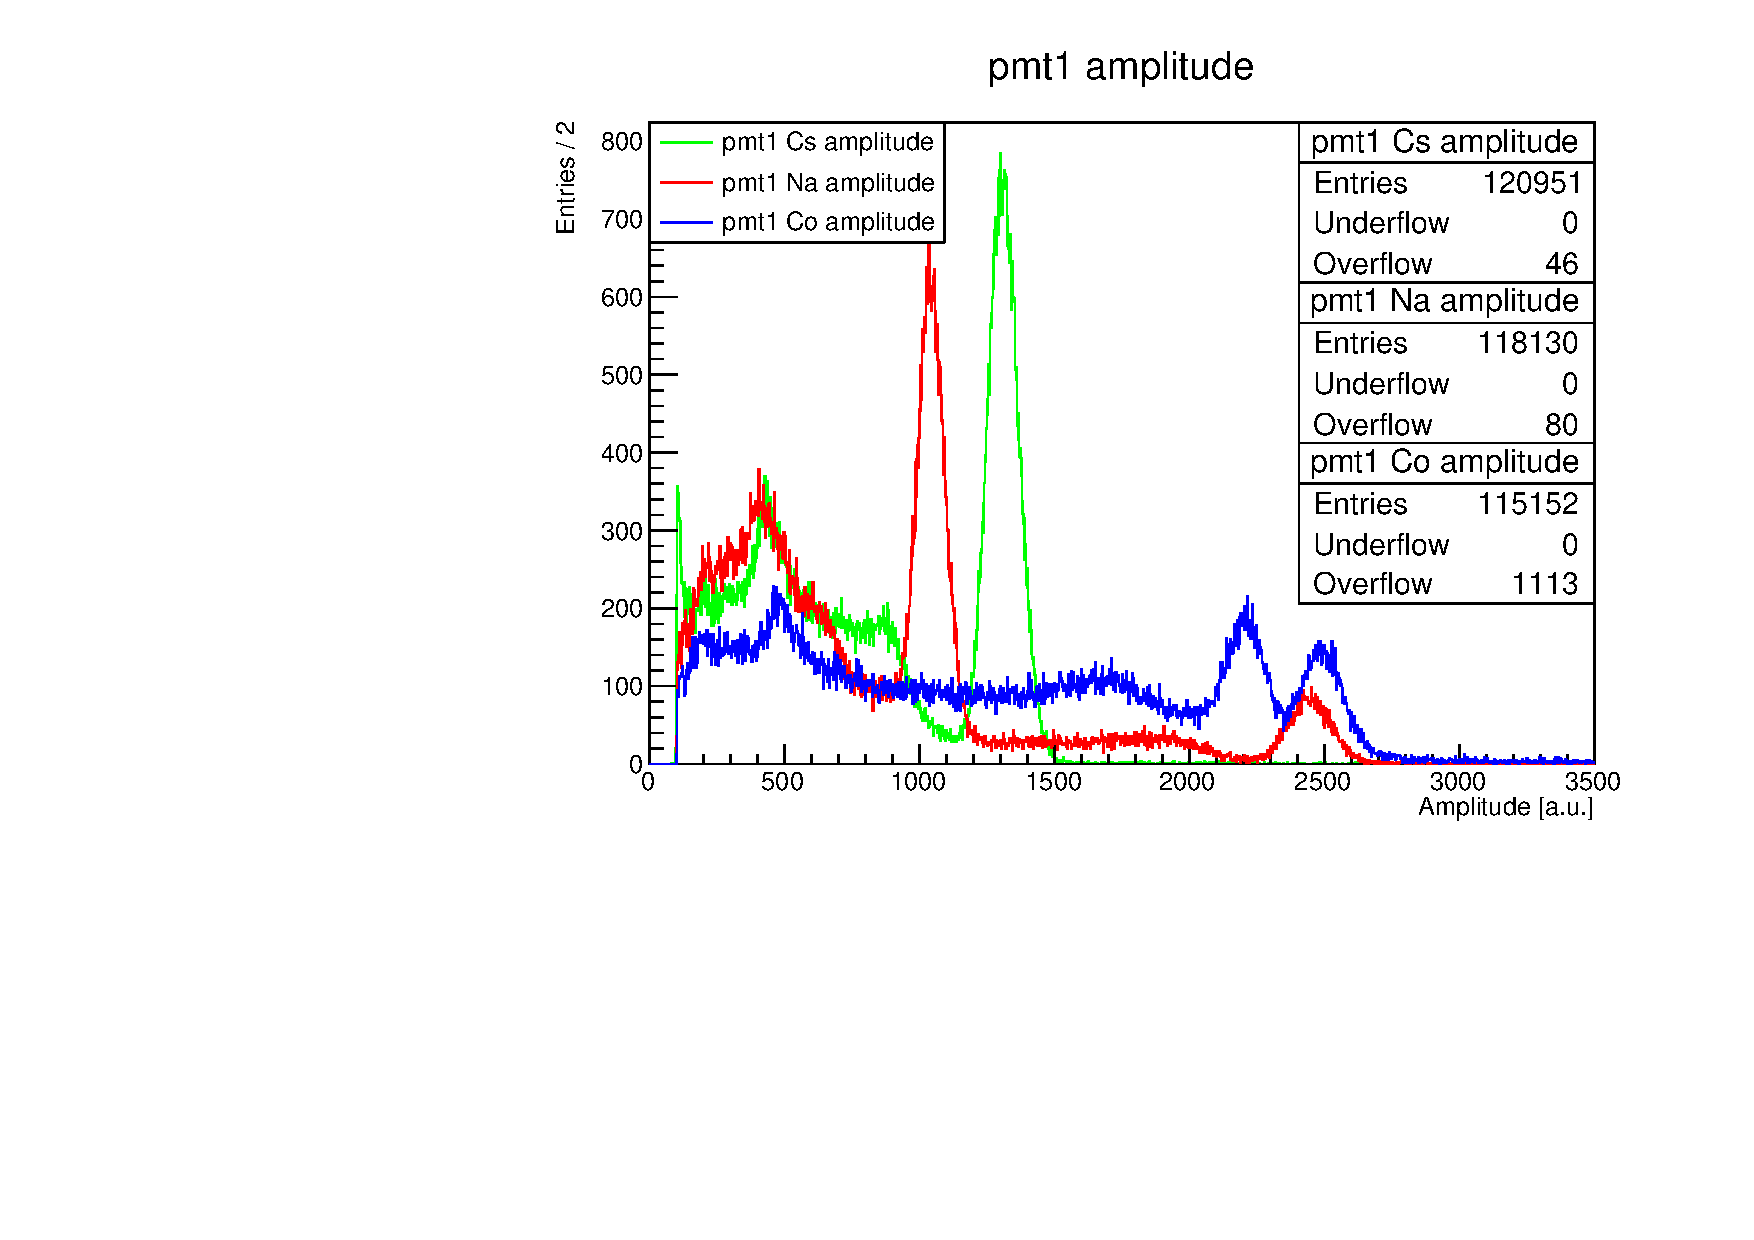
\includegraphics[scale=0.4]{Lab4/Positronio/pmt1_amp.pdf} 
\caption{$^{60}$Co, $^{137}$Cs and $^{22}$Na amplitude spectra.[Co: 03/03/22][Cs: 03/03/22][Na: 15/03/22]}
\label{fig:amplitudespectra}
\end{figure}

\section{TWO PHOTON DECAY}

The first objective of this work is actually measure a statistically significant presence of photons that travel back to back and have energy in the 511 KeV photopeak. Thanks to initial calibrations said photopeak is easily recognizable on the $^{22}$Na spectrum as the first peak after the first compton plateau. In order to observe back to back pairs of photons at the 511 KeV energy two NaI crystals (with their pmts) were placed on opposite sides of a stronger $^{22}$Na source. The latter was placed in the E6 cell of a "battleship" plastic grid, encased in an aluminium square box (see \figurename~\ref{fig:e6config}).

 \begin{figure}[h!]
\centering
\includegraphics[scale=0.15]{Lab4/Positronio/MicrosoftTeams-image(2).png} 
\caption{Configuration in which the source in placed in E6.[09/03/22]}
\label{fig:e6config}
\end{figure}

Using a discriminator NIM module, a dual timer NIM module, a coincidence NIM unit and the external trigger feature of the ADC converter it was possible to trigger on the coincidence of the two pmts. Unfortunately, unlike in the case of triggering on a single pmt, the ADC does not provide a way to internally trigger on the coincidence of multiple channels. For this reason it was necessary to create a coincidence signal to feed to the ADC. The use of the Dual Timer module was made necessary by the fact that the discriminator unit often sent two pulses for each waveform \footnote{This is due to the fact that by the time the discriminator updates its status, the input signal is still above threshold, thus the new output is still referred to the latter waveform.}. Therefore to avoid counting the same event twice the dual timer was used to artificially extend the duration of the discriminated signals (from  about 50 ns to about 500 ns). This way, in the event of a double pulse, the outcome would be a single signal, but of longer duration (usually around 750-800 ns). The time overlap allowed by the coincidence unit is by manual 2 ns, which is completely negligible compared to the length of these extended pulses as far as the later calculation of the expected frequency of random coincidences.

\noindent The discriminator thresholds were set to 

$$V^{thr}_{1}\simeq -32 \text{ mV}\quad , \quad V^{thr}_{2} \simeq -21 \text{ mV} $$
 
\noindent The choice for these thresholds was fairly arbitrary once it was verified that they allowed much of the compton plateau and even the backscatter peaks through. The thresholds on the discriminator couldn't be set to less than -10 mV in any case.
\\
\\
Two different approaches have been taken to demonstrate that there is in fact a correlation between photons at 511 KeV when back to back.

The first consists in veryifying that the probability of a 511 KeV photopeak event for pmt2 is greater if it is in coincidence with a photopeak event of pmt1 ($P_{2|1}$) than if it isn't correlated with pmt1 ($P_2$). The latter case consists of the probability of being in the photopeak if the events are triggered on the single pmt2 channel, without any coincidence involved. 
%In \figurename~\ref{fig:correlationintervals} the intervals which were regarded as 511 KeV photopeak are shown.

The results for the probability are \footnote{In this case the errors were calculated as if the events of interest were binomially distributed. In reality the number of events upon which these are normalized to calculate such probabilities are not fixed but instead Poissonian variables themselves. This method is therefore not correct and this is obvious in the limiting cases of P=0 or P=1, in which the uncertainty would be 0. Another approach way could be to use Ullrich and Zu's Bayesian approach, which yields similar results in this case. Of course these are unnecessary refinements since the two probabilities differ so wildly on sets of data of tens of thousands of events, so are clearly incompatible.}

$$ P_2= 0.257 \pm 0.001  \quad \quad \quad  P_{2|1}= 0.427 \pm 0.002$$

\noindent Since $ P_{2|1}$ is overwhelmingly greater than $P_2$ it is clear that the presence of a 511 KeV $\gamma$ is strongly linked to the presence of a similar $\gamma$ going in the opposite direction.

The second approach consists in measuring the number of events in which both pmts are hit by photons in their respective 511 KeV photopeaks ($N_{12}$) and comparing it to the one expected by random chance given the individual frequencies of such events on the two pmts separately ($N_{12}^{exp}$). This was done by triggering on either of the two pmts, directly with the ADC's internal trigger. The frequency expected for random coincidences is 

$$ f_{12}^{rdm}=f_1f_2\tau $$

\noindent where $f_1$ and $f_2$ are the individual frequencies of each pmt and $\tau = 4.12 \; \mu s$ is the time duration around the moment of trigger during which the ADC registers the signals \footnote{To be precise, the actual time duration that should be considered is not the whole interval of 4.12 $\mu s$ but only the fraction used for the computation of the charge/amplitude (about 2.6 $\mu s$), since outside of this range the events are discarded. Moreover, the time duration of the signal ($\sim $700 ns) should be added twice. However, a overestimate can be obtained by simply considering the whole interval which is more than enough for this purpose.}.
Finally to obtain $N_{12}^{rdm}$ 


\begin{equation}
    \label{eqn:N12rdm}
    N_{12}^{rdm}=  f_{12}^{exp} \Delta T=f_1f_2\tau \Delta T
\end{equation}
 

\noindent where $\Delta T$ is the total time during which the events were recorded.

\noindent The final results are

$$ N_{12}^{rdm}= 33.5 \pm 0.3 \quad \quad \quad N_{12}= (3.56 \pm 0.06) \cdot 10^3  $$

\noindent The goal is to compare the two distributions, the one of the actual number of coincidences and the one of random coincidences, which is all that would be expected if the events were not correlated. Since these are poissonian by nature, their expected values are compared. However it is impossible to know the value of these expected values: the two numbers reported are precisely estimators of these means. The errors reported are therefore the standard deviations of the \textit{estimators}. A more in depth analysis on how the uncertainties were obtained is found in Appendix \ref{appendix:N_uncertainties}.

These results once again clearly show that the presence of one photon positively correlates with the presence of the other.
\\
\\
Using the data acquired in this stage it is also possible to prove that the when the annihilation happens the electron and the positron are essentially still in the lab frame, at least to the order of $\beta_{cm} \sim T/m_e$. To see this two intervals on the 511 KeV photopeak have been taken for the two pmts in coincidence triggering. Then the energies of the photons belonging to an event in which both photons are in the respective intervals were plotted one against the other in a scatterplot. Finally, these points where linearly fitted to find a correlation between the two energies (\figurename~\ref{fig:energycorrelationscatter}).
 
\begin{figure}[h!]
\centering
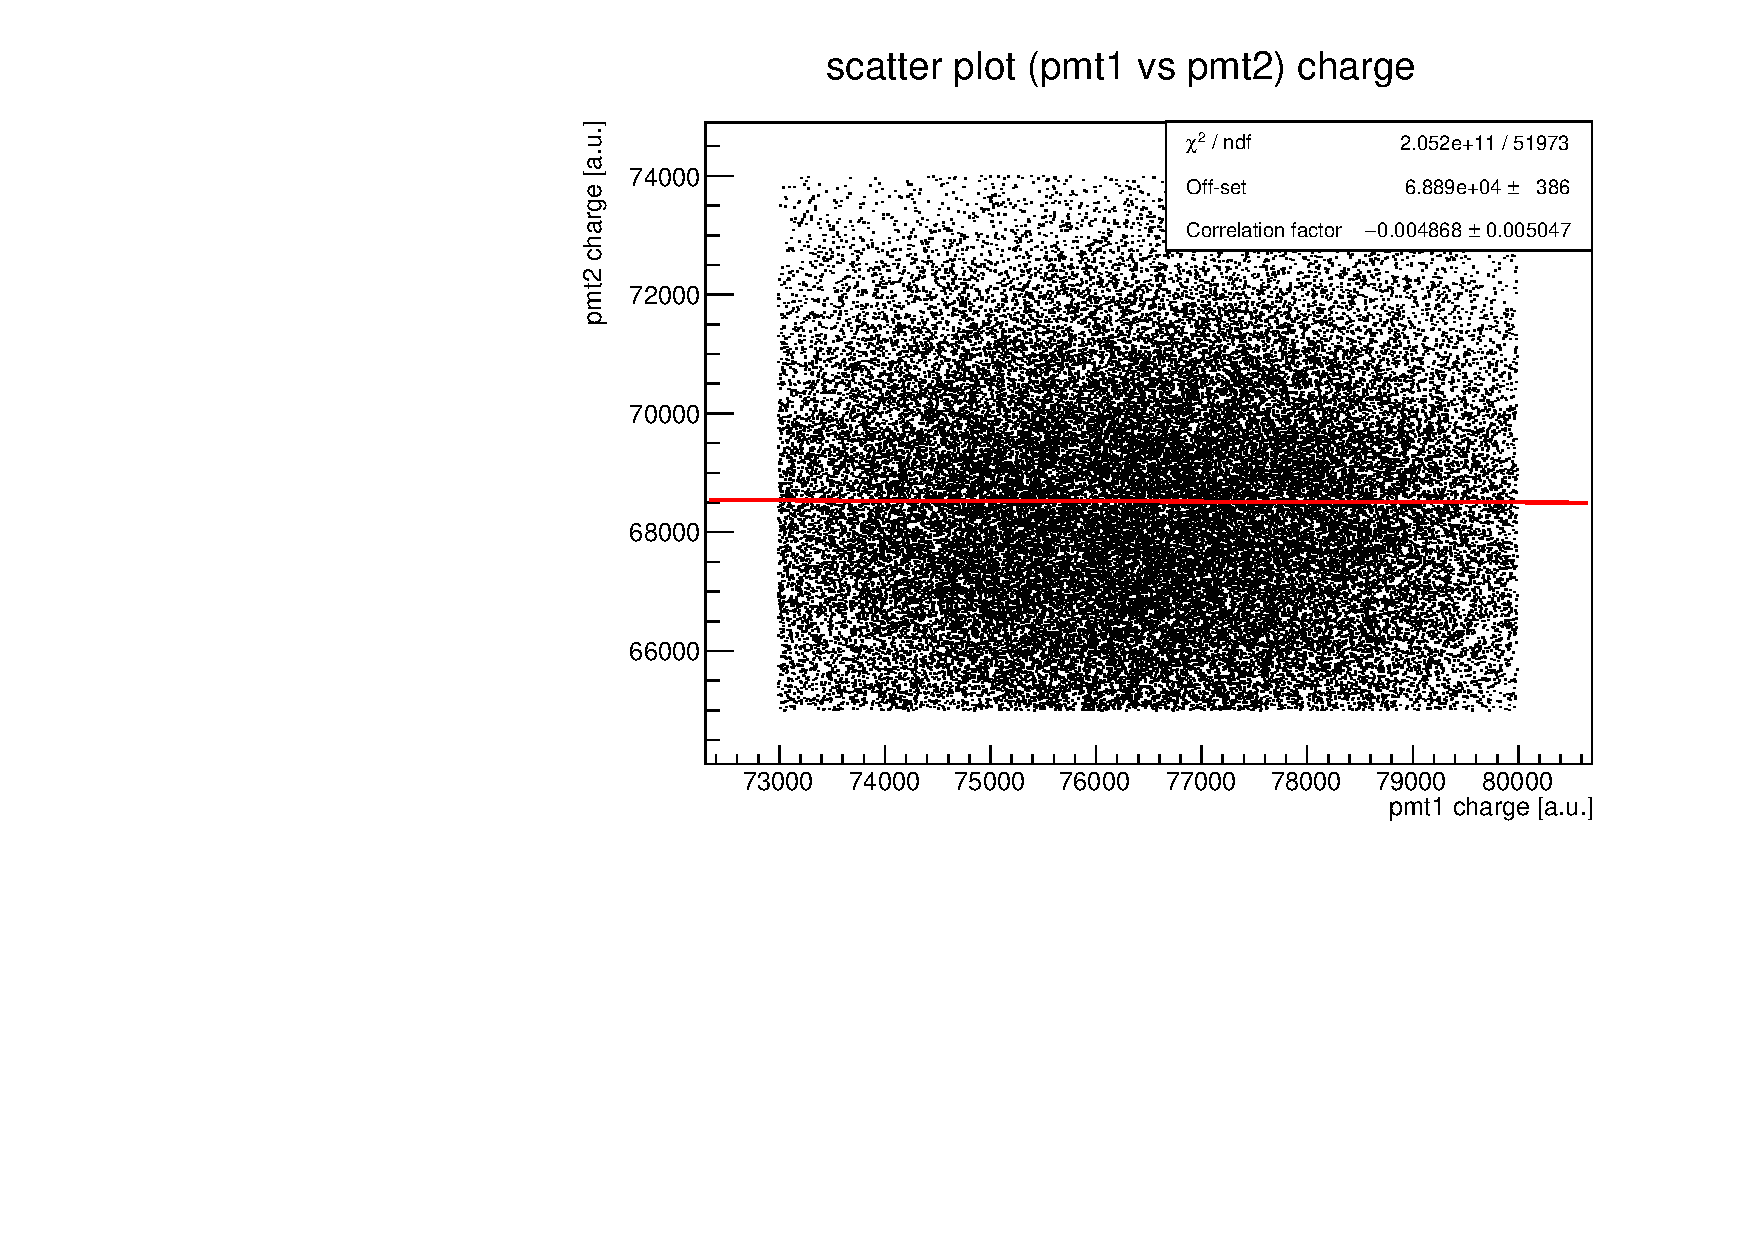
\includegraphics[scale=0.45]{Lab4/Positronio/scatter.pdf} 
\caption{$^{22}$Na charge scatter plot pmt1 vs pmt2.
[8/03/22]}
\label{fig:energycorrelationscatter}
\end{figure}

\noindent Since the correlation found was compatible with zero any fluctuation above or below the peak average of the charge generated by these photons is solely due to the resolution of the apparatus, not to the fact that if one of the photons has more energy the other has less. The latter result, in which a negative correlation would have been observed, is to be expected if the $e_+e_-$ pair annihilates in motion with respect to the lab. In that case the photons have same energy in the pair reference frame and therefore have different energies in the boosted lab frame.




\section{MEASUREMENT OF $m_e$}
Initially, the spectra of $^{60}$Co, $^{137}$Cs and $^{22}$Na were measured separately.
However, the charge corrisponding to the same peaks was observed to change in measurements done on different days, by much more than the statistical uncertainty of the position of such peaks. For instance in \figurename~\ref{fig:sodiumdiscrepancy} this variation is visible in the $^{22}$Na spectrum and it is more than 10 times the fit uncertainty of the peak location. 
 
 
\begin{figure}[h!]
\centering
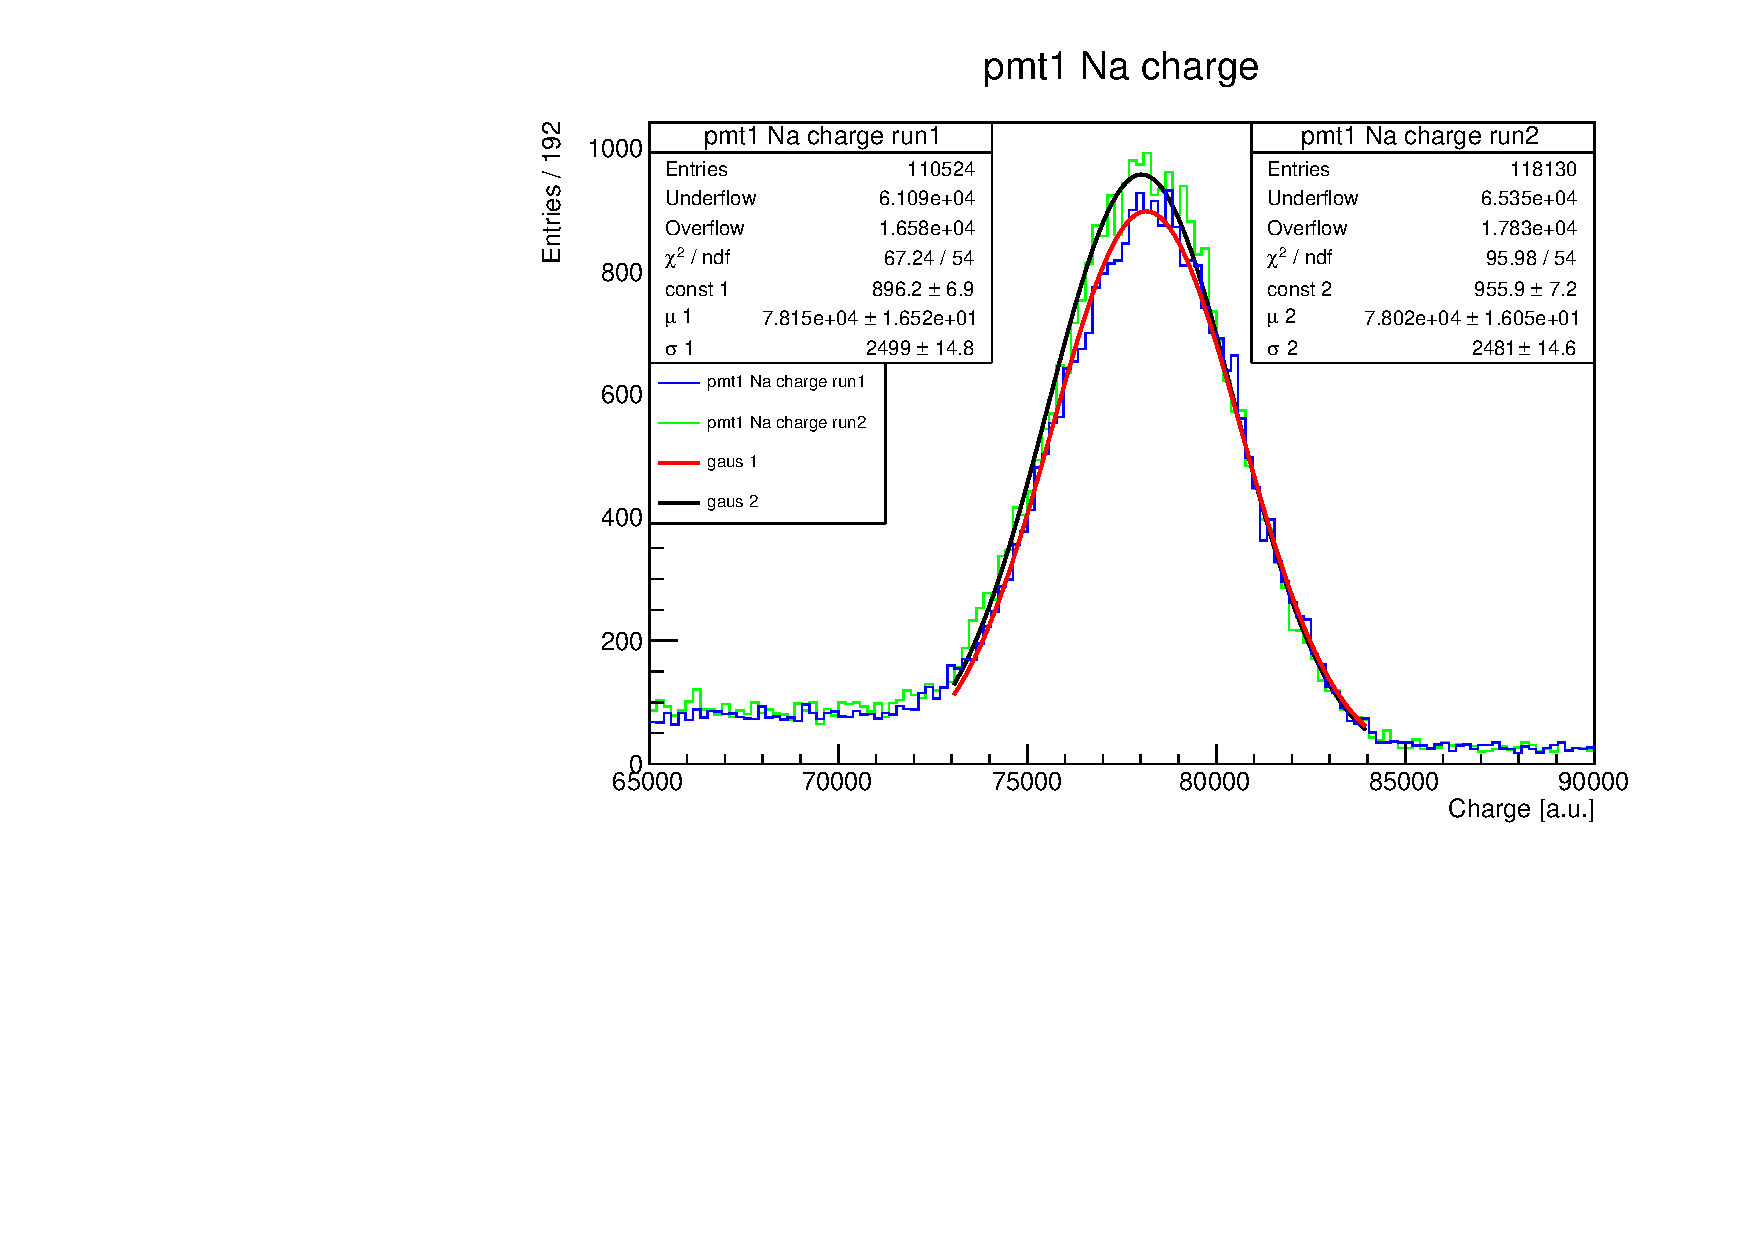
\includegraphics[scale=0.4]{Lab4/Positronio/pmt1_Na_charge.pdf} 
\caption{$^{22}$Na charge spectrum measured in two separate runs.
[run1: 03/03/22][run2: 15/03/22]}
\label{fig:sodiumdiscrepancy}
\end{figure}

In order to eliminate or at least reduce this effect due to unknown fluctuations in time, a real time calibration was performed for the final $m_e$ measurement, with multiple sources of radiation present in the system at the same time. 

The main issue with this approach is that the Ne photopeak in the Na spectrum (1.274 MeV) is right in the middle of the two photopeaks of the Co spectrum (1.173 Mev and 1.333 MeV). Given the resolution of the system these peaks merge together, especially the ones 1.274 MeV and 1.333 MeV. For this reason it was necessary to measure the spectra with Na+Cs and Na+Cs+Co separately and then subtract the Ne peak found on the one without Co from the one with Co (see \figurename~\ref{fig:realtimecalib}). This procedure was executed twice, on two different days, for each of the three pmts, leading to 6 distinct measurements of $m_e$ using charge and 6 using the amplitude.

\begin{figure}[h!]
\centering
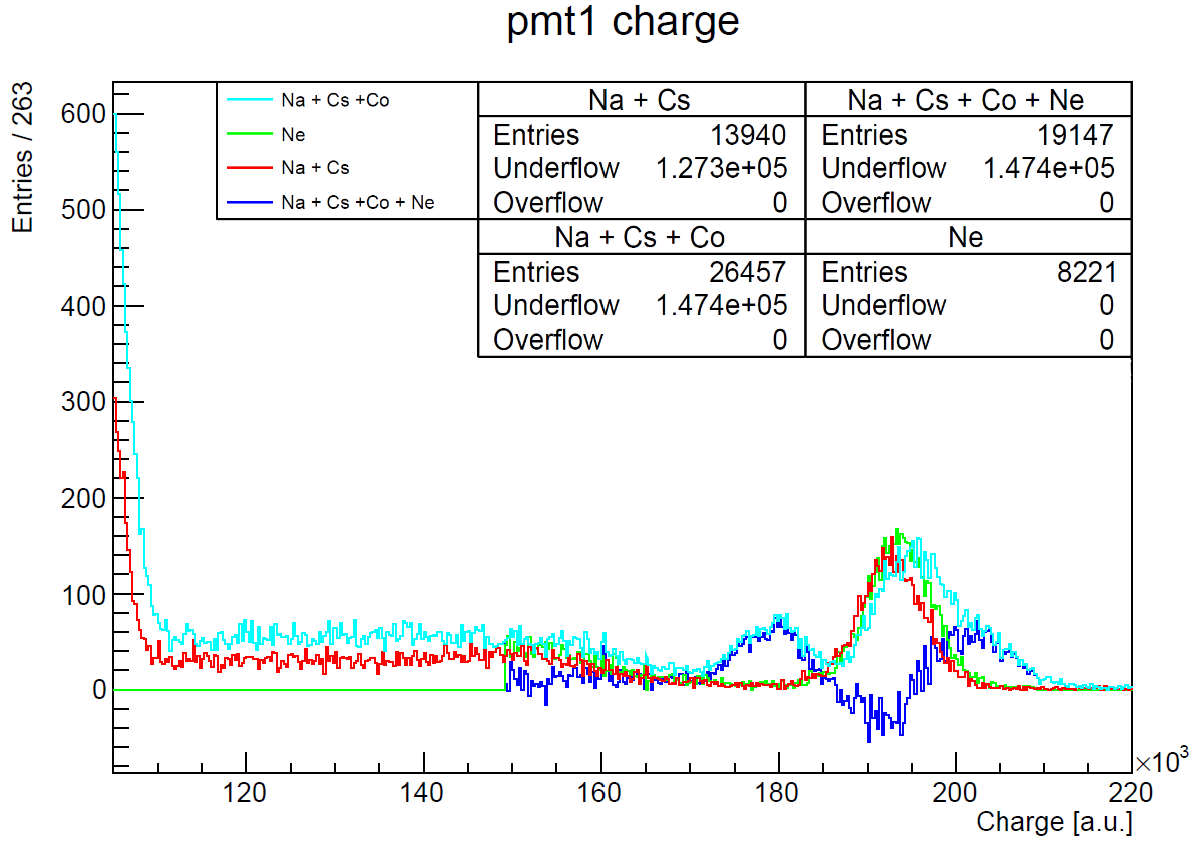
\includegraphics[scale=0.25]{Lab4/Positronio/pmt1_all.png} 
\caption{pmt1 charge spectrum. [16/03/22]}
\label{fig:realtimecalib}
\end{figure}

Another issue observed is that \textit{in the same run} the positions of the same peaks changed between the Co and the no Co case, even by as much as 1\%, 1-2 orders of magnitude above the statistical peak uncertainty (\figurename~\ref{fig:intrarundiscrepancy}).This effect cannot be due to fluctuations in time of the pmt calibration like the one noted at the beginning of this section. It could be due to other effects, such as a slight dependency of the calibration factor from the rate of events (which of course changes if Co is added to the already present sources). However this effect is not present in the case of pmt3 (\figurename~\ref{fig:pmt3norundiscrepancy}), so either the pmts have different behaviors in this aspect or the change in rate is not the cause for this effect. For this reason when necessary the spectrum was shifted accordingly when subtracting the Ne peak. This is one of the causes for systematic error that shall be considered later.

\begin{figure}[h!]
\centering
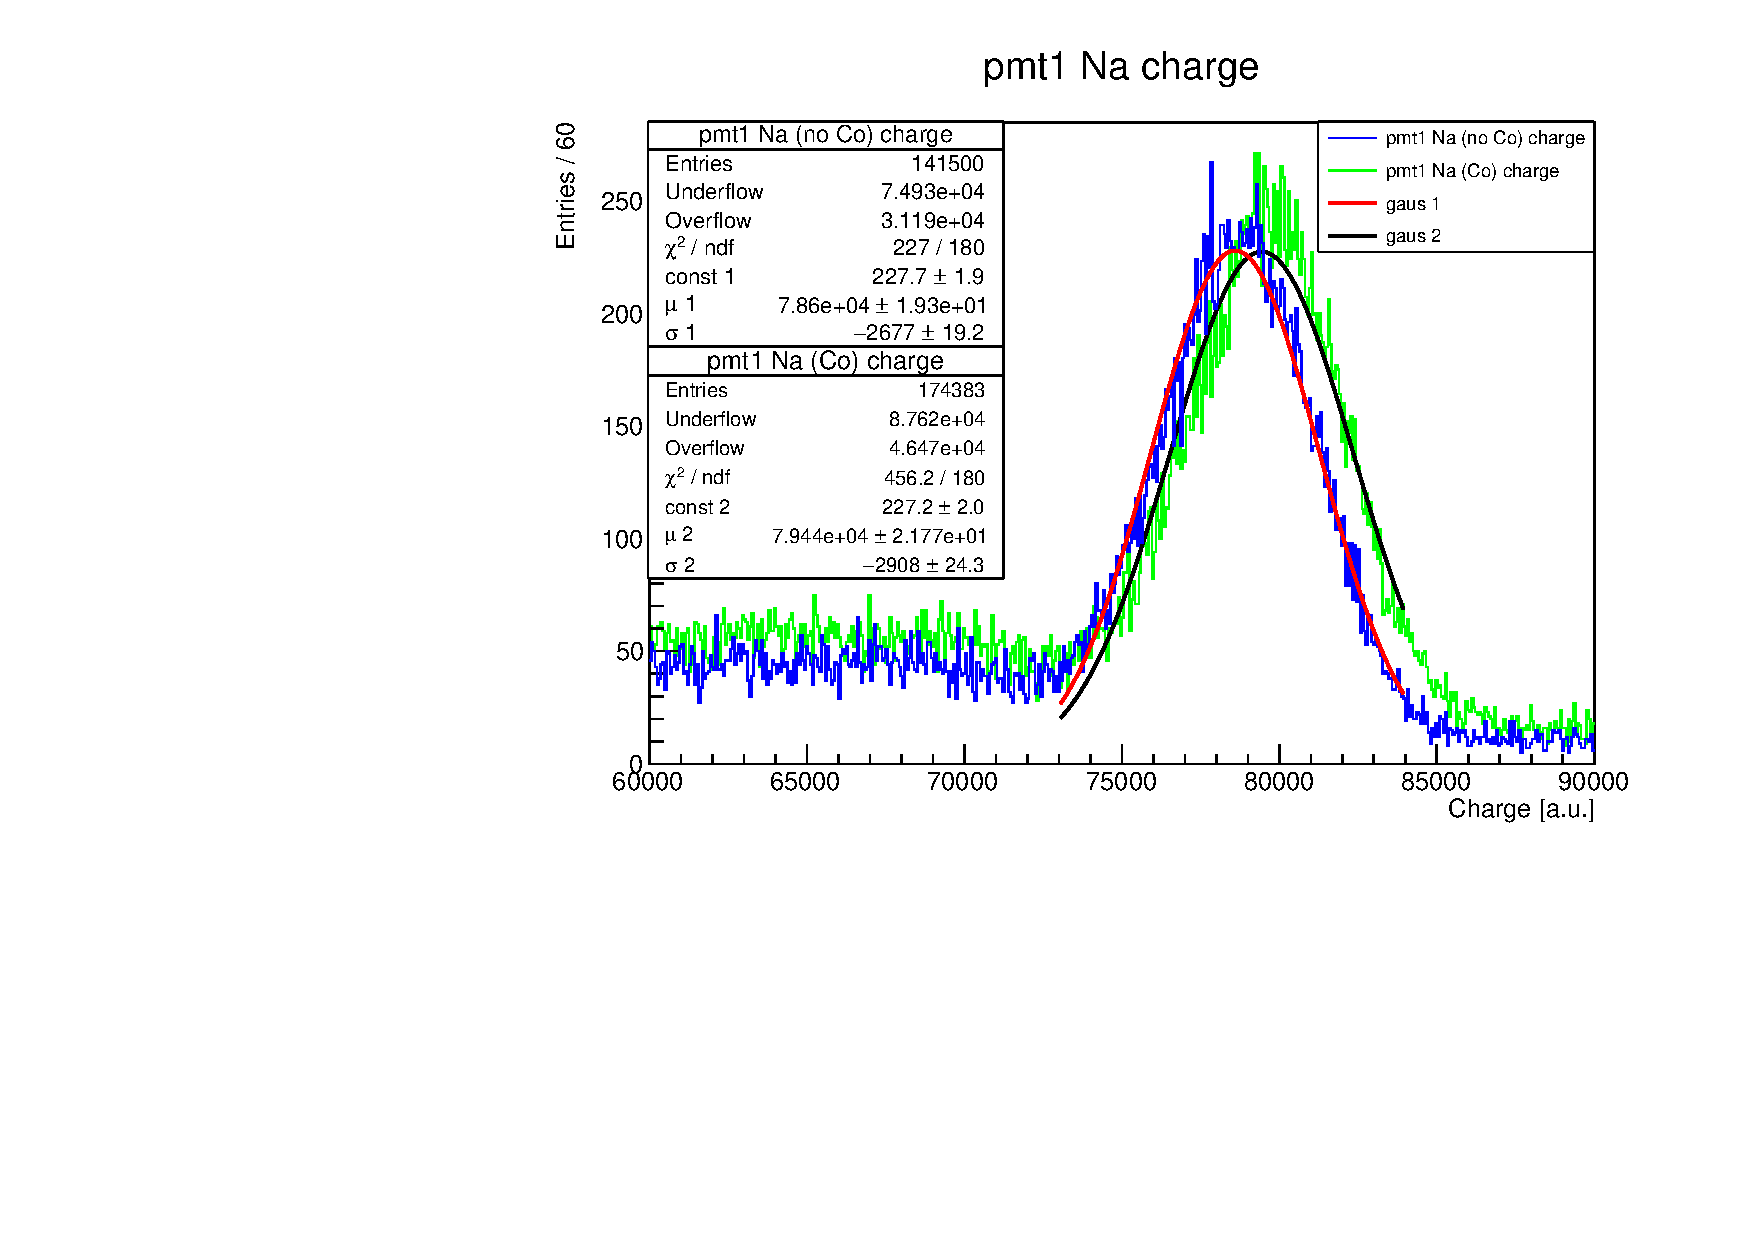
\includegraphics[scale=0.43]{Lab4/Positronio/pmt1_Na(csvsco)_charge.pdf} 
\caption{pmt1 Na charge spectrum with and without Co. [16/03/22]}
\label{fig:intrarundiscrepancy}
\end{figure}

\begin{figure}[h!]
\centering
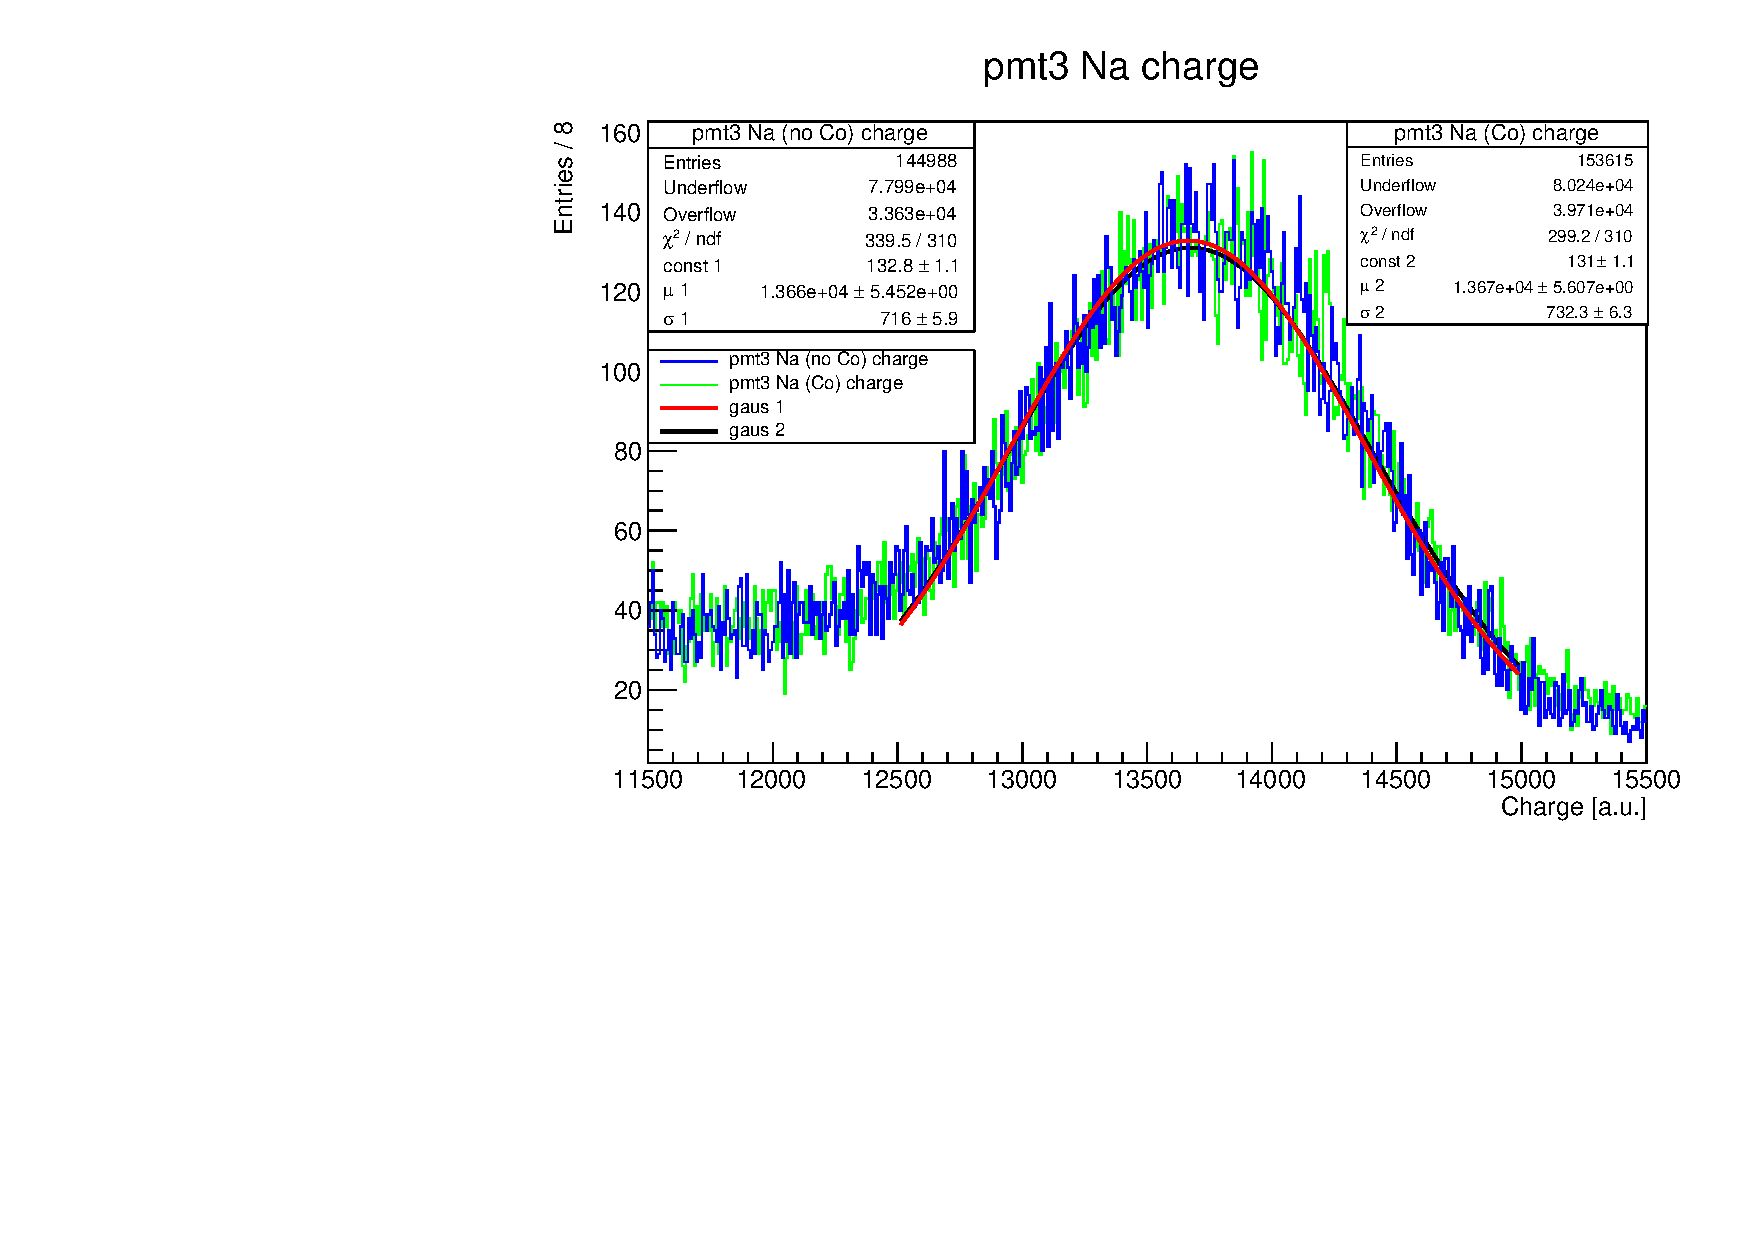
\includegraphics[scale=0.43]{Lab4/Positronio/pmt3_Na(csvsco)_charge.pdf} 
\caption{pmt3 Na charge spectrum with and without Co. [16/03/22]}
\label{fig:pmt3norundiscrepancy}
\end{figure}

\noindent Once the positions of the peaks were measured in a.u. they were fitted with a linear model, having assigned each point the statistical uncertainty given by the gaussian fit of the peaks.  An example of such fits is given in \figurename~\ref{fig:realtimecaliblinfit}.
In these fits the Ne peak was not used because of the shift mentioned earlier: all the peaks measured (Na 511, Cs and the two Co) were all taken from the same condition (the one with Co of course) for this very reason.
The 6 measurements of the masses are reported in \figurename~\ref{fig:realtimecaliblinmass}. As we can see, the various estimates are compatible with each other but are around 507 KeV, not the PDG value of the electron mass (511.0 KeV).

\begin{figure}[h!]
\centering
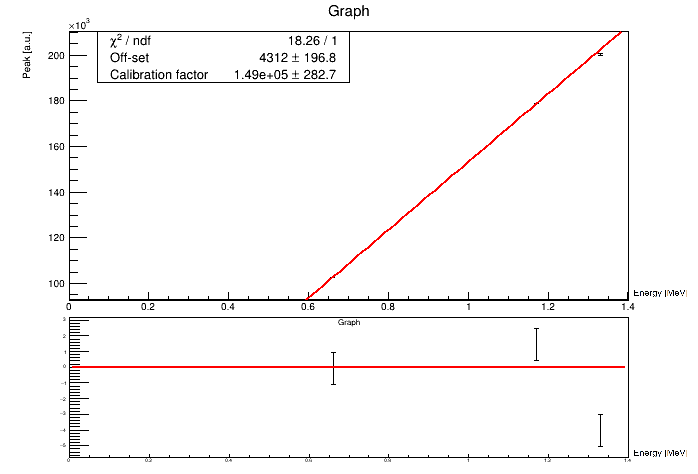
\includegraphics[scale=0.4]{Lab4/Positronio/fit_lin.png}
\caption{Linear fit of the charge peaks as a function of the energy of the peaks. [16/03/22]}
\label{fig:realtimecaliblinfit}
\end{figure}


\begin{figure}[h!]
\centering
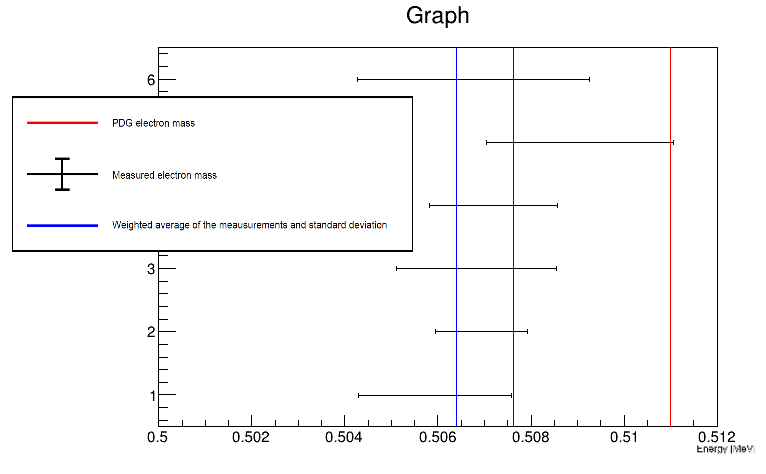
\includegraphics[scale=0.4]{Lab4/Positronio/mass_lin.png}
\caption{Electron mass estimate obtained with the charge and linear model. The various points are, from top to bottom, the two estimates obtained from the two runs of pmt3, pmt2 and pmt1. [17/03/22]}
\label{fig:realtimecaliblinmass}
\end{figure}



The most evident cause of discrepancy between the measured masses and the PDG value is the fitting model used. By using a linear fitting model the constant term was found to be far from null (around 3000-4000 in fact). But measuring the charge spectrum of flat (no event) waveforms the results are as show in \figurename~\ref{fig:nullcharge}: random noise, corresponding to zero energy, has on average less than 10 a.u. of charge, and its standard deviation is only around 400 . This could indicate a non linearity in the actual calibration of the detector. 

\begin{figure}[h!]
\centering
\includegraphics[scale=0.25]{Lab4/Positronio/pmt1_nullcharge.png}
\caption{pmt1 charge spectrum in absence of signal. [02/03/22]}
\label{fig:nullcharge}
\end{figure}

For this reason the same procedure was repeated but with a quadratic model (next term in Taylor expansion), imposing that the constant term be zero. An example of such fit is reported in \figurename~\ref{fig:realtimecalibquadfit} and the final mass measurements for charge and amplitude in \figurename~\ref{fig:realtimecalibquadmass_charge}~\ref{fig:realtimecalibquadmass_amp}. In \figurename~\ref{fig:realtimecalibquad_ne_charge} ~\ref{fig:realtimecalibquad_ne_amp} the estimates for the Ne energy are reported as well.

\begin{figure}[h!]
\centering
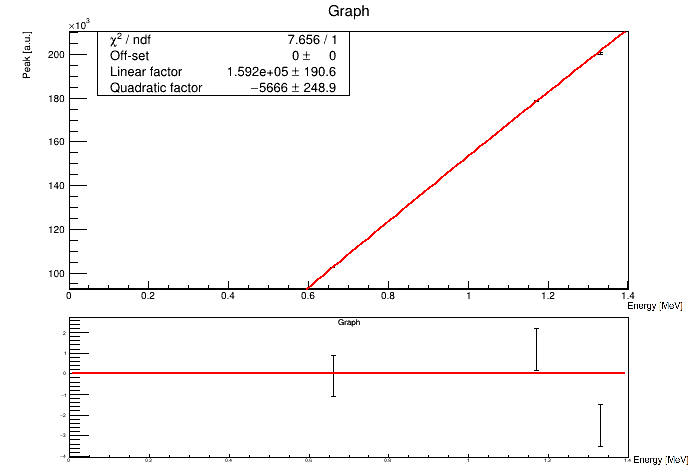
\includegraphics[scale=0.4]{Lab4/Positronio/quad_fit.png}
\caption{Quadratic fit of the charge peaks as a function of the energy of the peaks. [16/03/22]}
\label{fig:realtimecalibquadfit}
\end{figure}

\begin{figure}[h!]
\centering
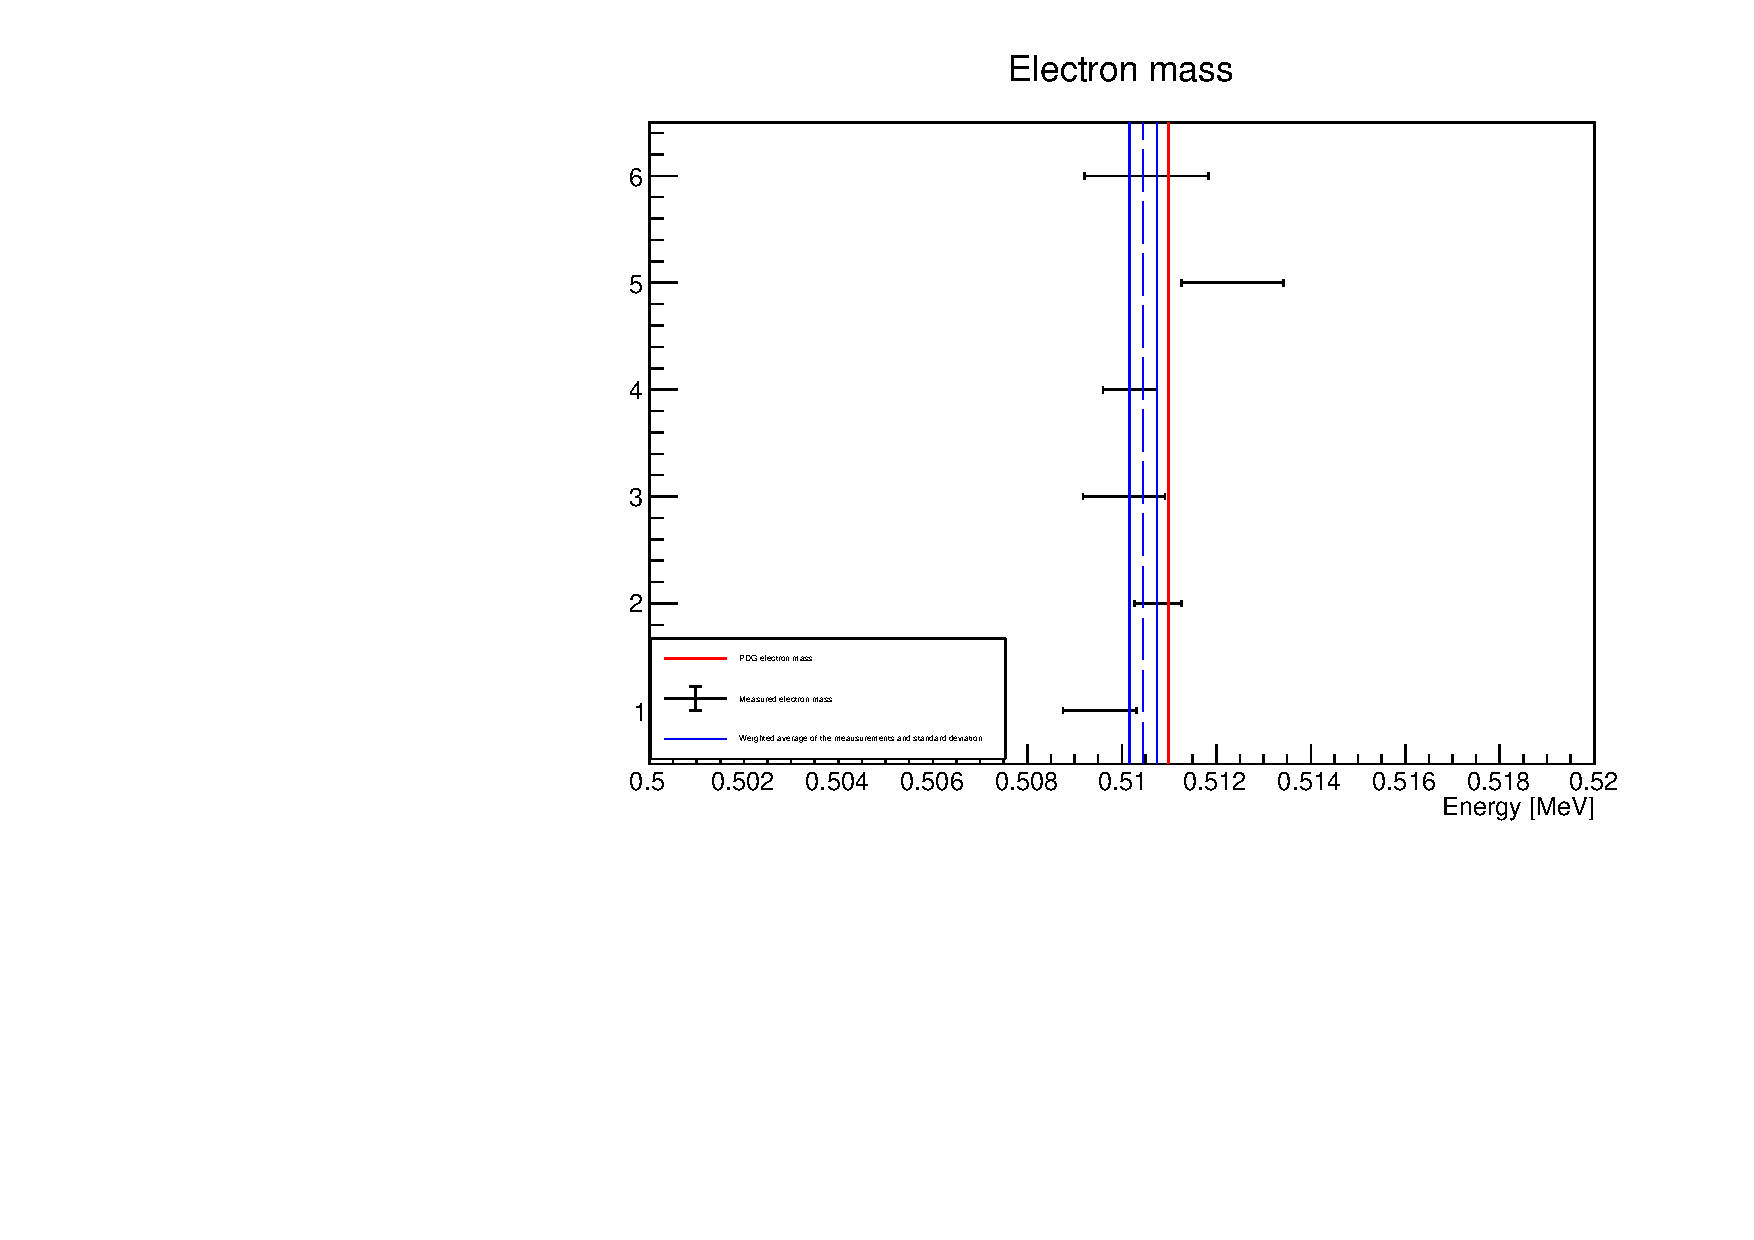
\includegraphics[scale=0.4]{Lab4/Positronio/mass_charge.pdf}
\caption{Electron mass estimate obtained with the charge. The various points are, from top to bottom, the two estimates obtained from the two runs of pmt3, pmt2 and pmt1. [17/03/22]}
\label{fig:realtimecalibquadmass_charge}
\end{figure}

\begin{figure}[h!]
\centering
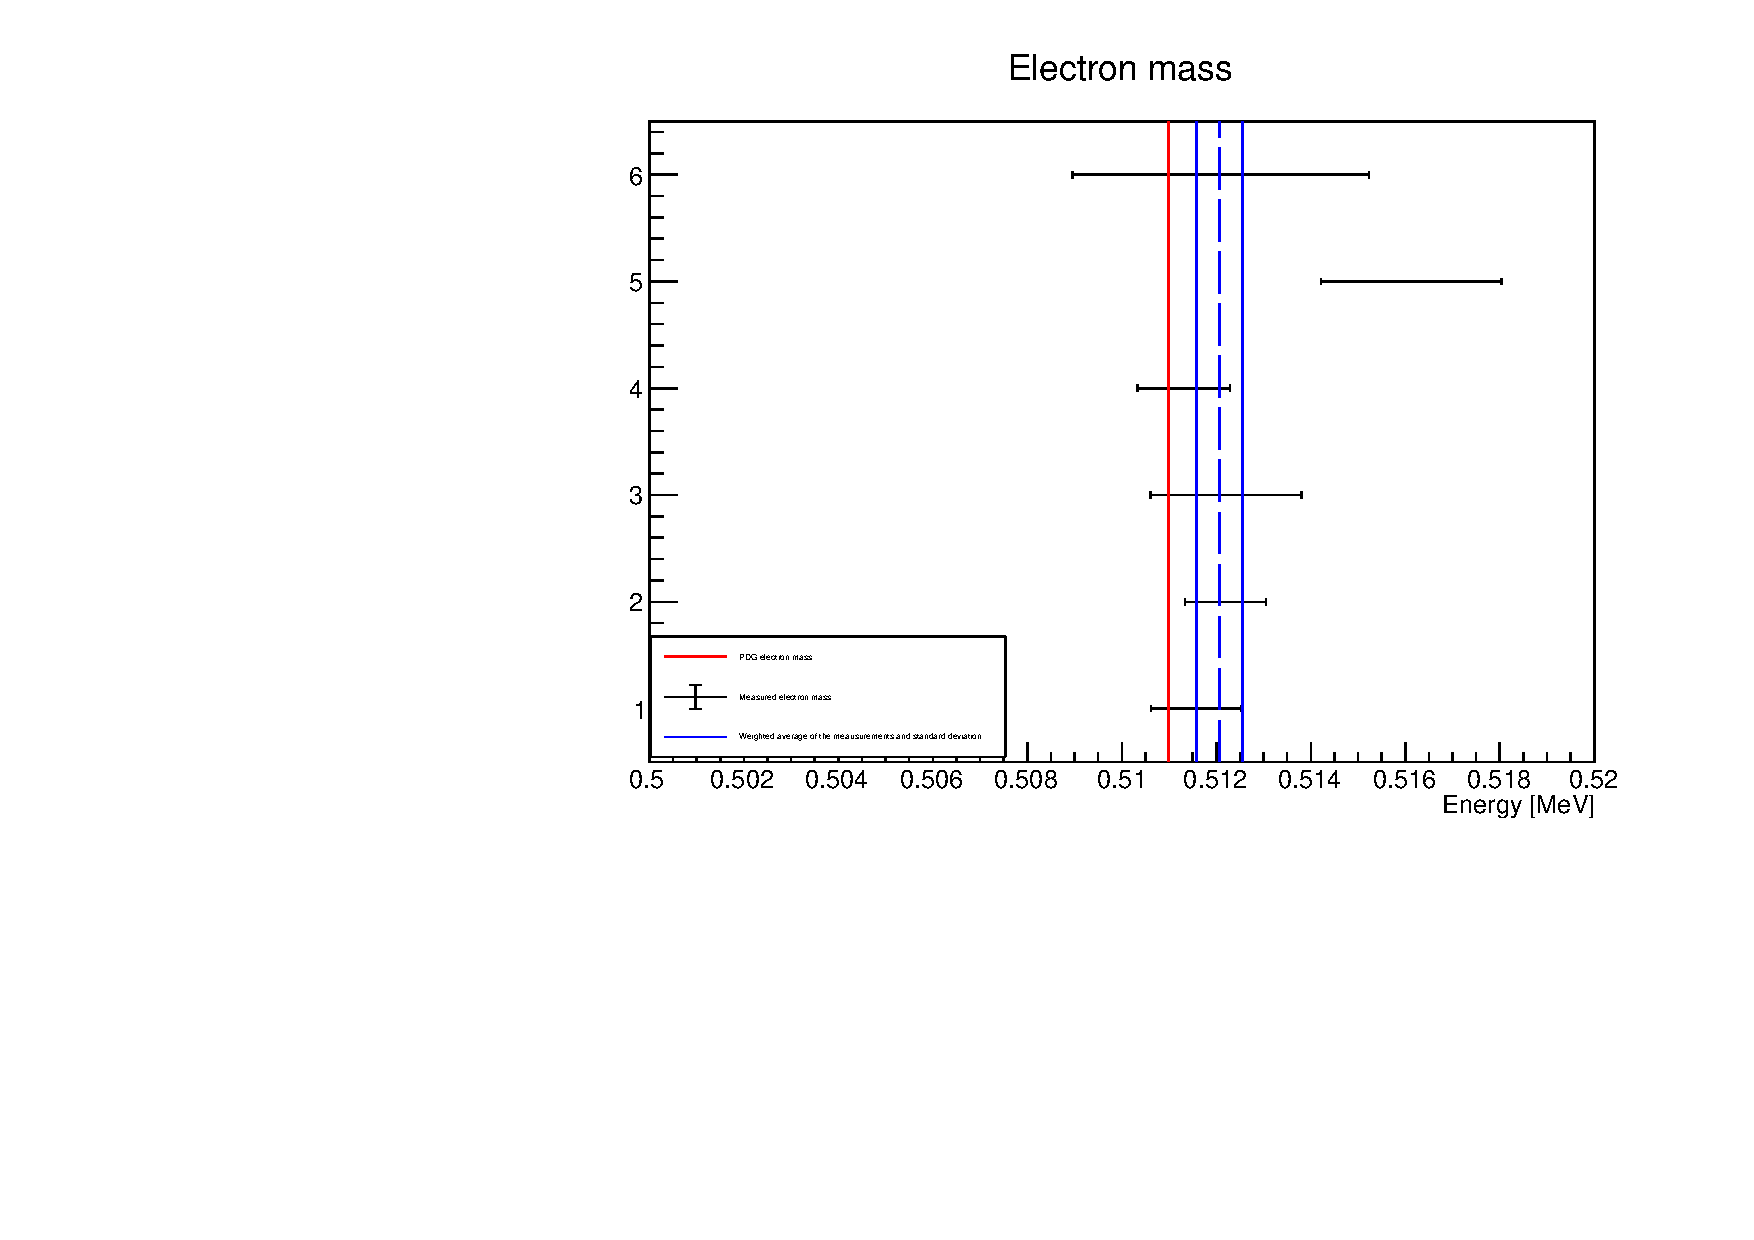
\includegraphics[scale=0.4]{Lab4/Positronio/mass_amp.pdf}
\caption{Electron mass estimate obtained with the amplitude. The various points are, from top to bottom, the two estimates obtained from the two runs of pmt3, pmt2 and pmt1. [17/03/22]}
\label{fig:realtimecalibquadmass_amp}
\end{figure}

\begin{figure}[h!]
\centering
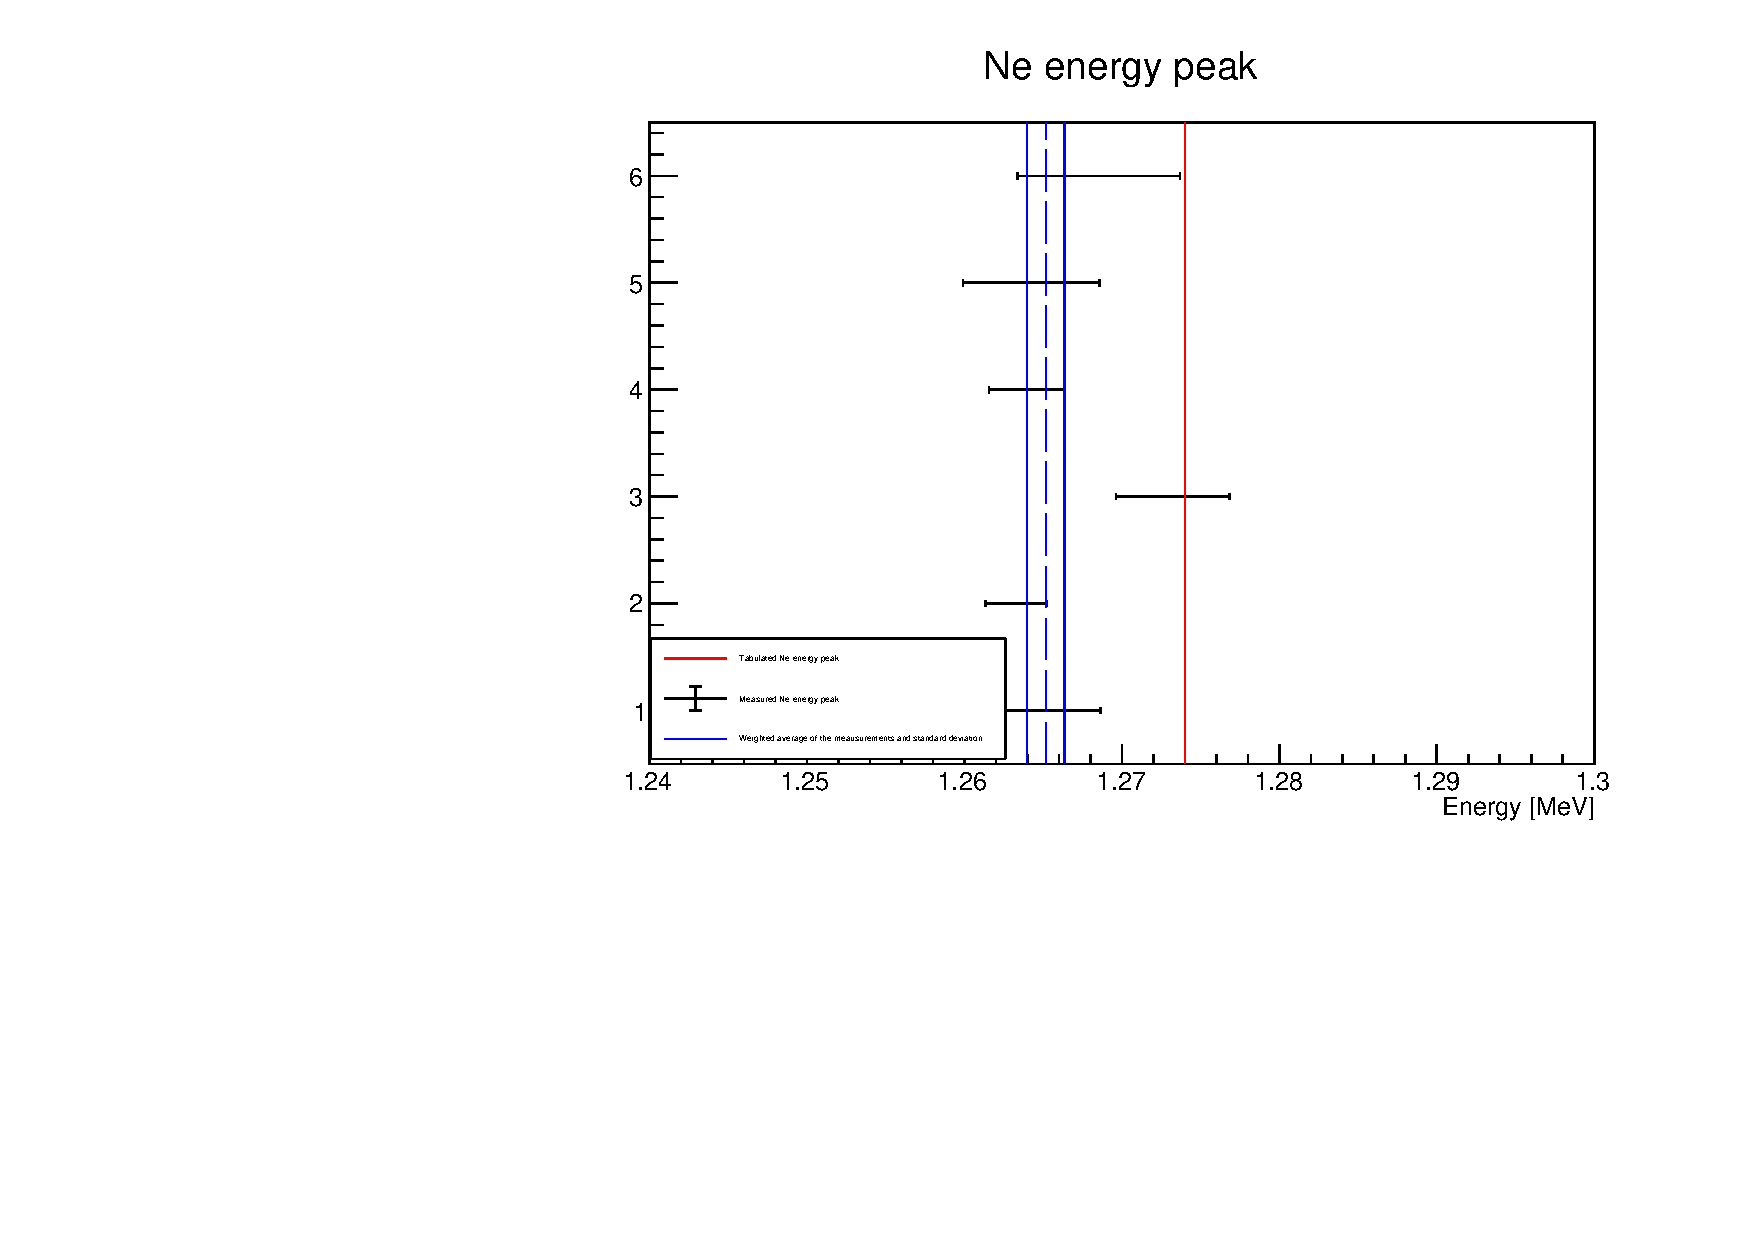
\includegraphics[scale=0.4]{Lab4/Positronio/ne_charge.pdf}
\caption{Ne peak estimate obtained with the charge. The various points are, from top to bottom, the two estimates obtained from the two runs of pmt3, pmt2 and pmt1. [17/03/22]}
\label{fig:realtimecalibquad_ne_charge}
\end{figure}

\begin{figure}[h!]
\centering
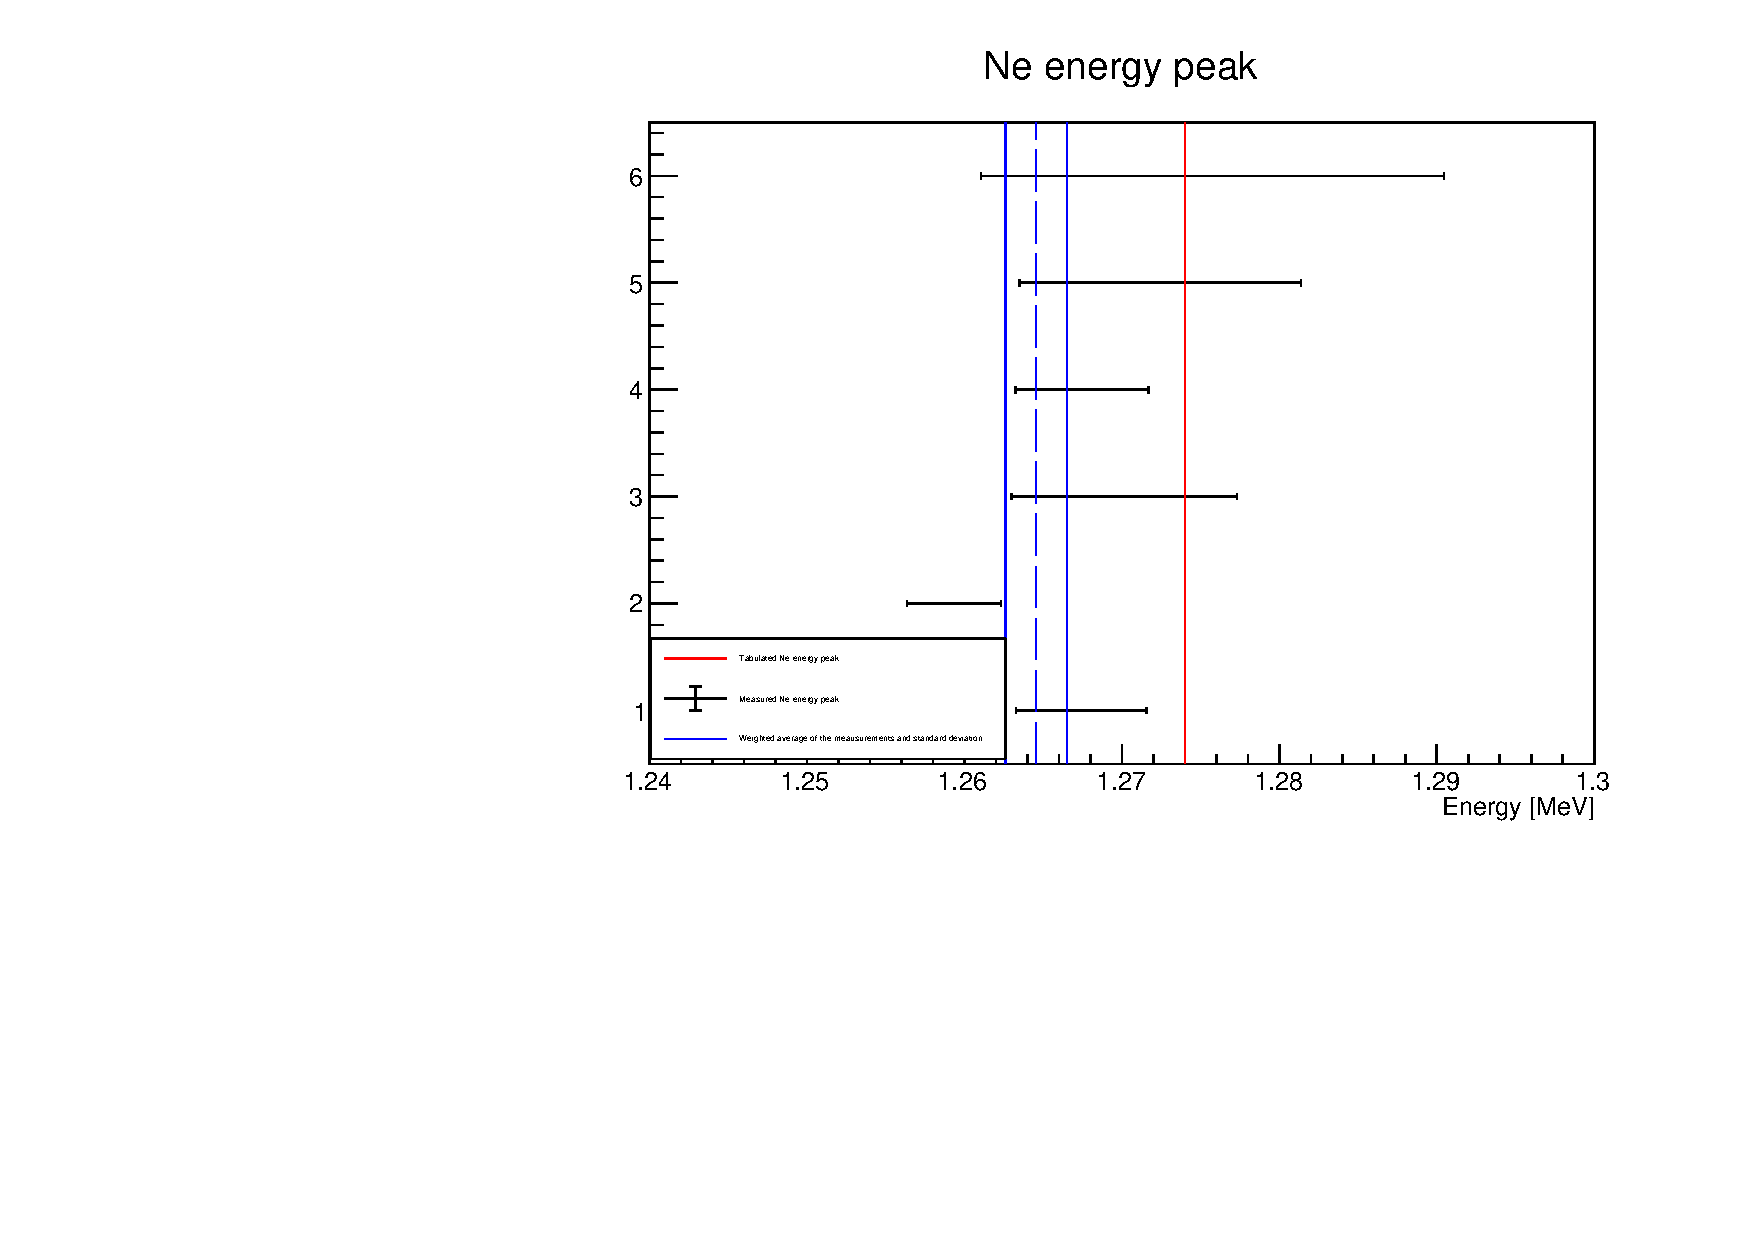
\includegraphics[scale=0.4]{Lab4/Positronio/ne_amp.pdf}
\caption{Ne peak estimate obtained with the amplitude. The various points are, from top to bottom, the two estimates obtained from the two runs of pmt3, pmt2 and pmt1. [17/03/22]}
\label{fig:realtimecalibquad_ne_amp}
\end{figure}

In order to estimate the systematical uncertainty of the mass measurement, other fitting methods were considered. First of all the histograms were also fitted after shifting the Ne peak accordingly to the rest of the spectrum since, as explained before, there is a discrepancy from the data with and without Co. Furthermore, a fit with a Gaussian summed with a constant function model was executed in order to consider the presence of the pedestal. At this point the semi-difference between the two more distant measurements was taken as the systematic uncertainty and the mean of these results as the central value. The final measurement of the electron mass obtained with the charge is 

\begin{equation}
    m_e=510.1 \pm 0.5 \text{ (sys)} \pm 0.3 \text{ (stat) KeV} 
\end{equation}

\noindent This is compatible with the PDG value of 511.0 KeV within just over one error bar.
\\
\\
The measurements with charge were not merged with the ones with amplitude because they are surely correlated and we do not know exactly how. They are however compatible within a margin of two error bars.

An aspect that should be further investigated is the fact that the Ne energy was \textit{not} found to be compatible with the PDG value. This could be due to the fact that the part of the calibration curve that concerns the Ne peak is the one that is between the Co peaks, which carry the most uncertainty being derived from a spectrum subtraction.



\section{3$\gamma$ DECAY RATE}

When $e^+$ and $e^-$ collide and annihilate there is also a smaller chance of them producing \textit{three} photons. Being this a three body decay, their energies and relative angles are not fixed but can instead vary inside of certain bounds. The objective is observing these events, distinguishing them from the much more abundant background (given the fact that $\alpha$ is of the order of $10^{-2}$, at least a similar ratio of signal to noise is expected). To do so, the pmts were arranged in a "Mercedes" composition (\figurename~\ref{fig:mercedes}) and the trigger was set on the coincidence of pmts 1 and 2, which are the ones on the above and below respectively in the picture. The relative distances of the pmts are such that the angles between pmt1-pmt2 and pmt1-pmt3 are respectively \footnote{The uncertainties are calculated as absolute uncertainty. For the measurements from which these angles are derived tape measure was used. The measures of the lengths were not very precise (about 1\% relative error) due to experimental constraints, such as the lead wall between the source and the lab, that induced parallax error in the readings}

$$\xi_{12}= 118.8 \pm 3.5 \text{ Deg} \quad \quad \xi_{13}= 120.6 \pm 0.9 \text{ Deg} $$


 \begin{figure}[h!]
\centering
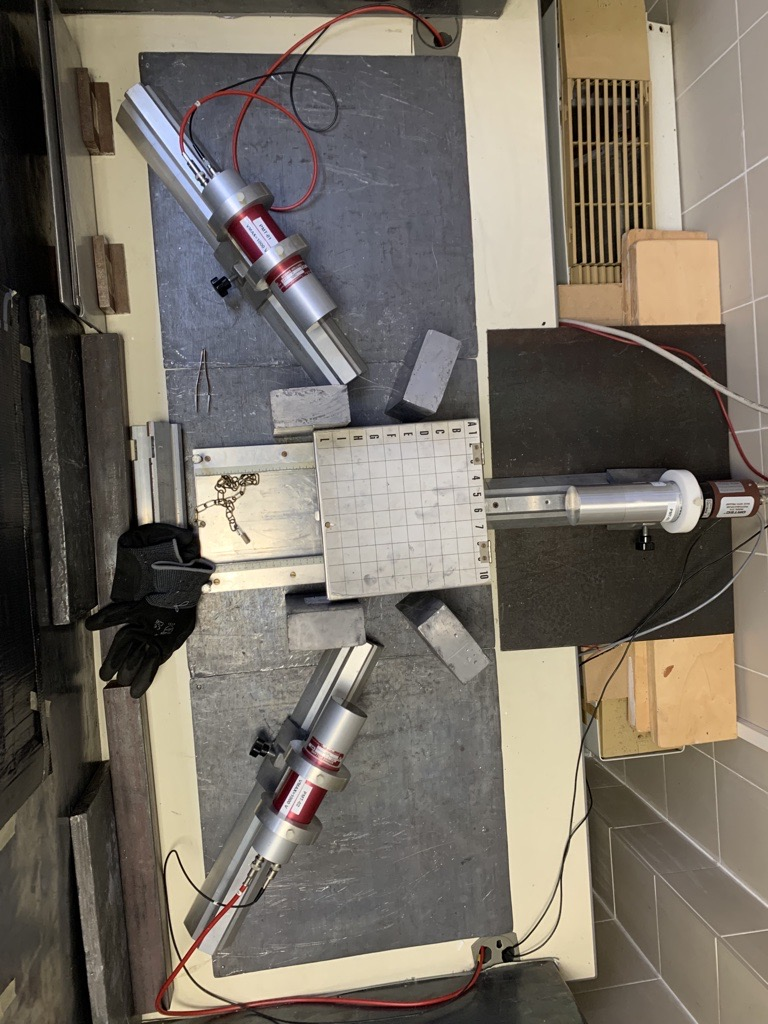
\includegraphics[scale=0.2]{Lab4/Positronio/MicrosoftTeams-image.png} 
\caption{"Mercedes" configuration in which the source in placed in C1.[30/03/22]}
\label{fig:mercedes}
\end{figure}

The pmts couldn't be placed nearer to the source, which was in the C6 cell, because of the constraints on the shielding. This was obtained with the lead blocks visible in the picture. Such shielding is necessary to eliminate or at least vastly suppress events in which the annihilation is $\gamma \gamma$ but the two photons are able to hit two pmts and events in which the same $\gamma$ ricochets off one pmt due to compton effect and subsequently hits another one. In this configuration the frequency of events triggered was very low (around 1 Hz) compared to earlier configurations (with frequencies of $10^2-10^3$ Hz).

In \figurename~\ref{fig:c1mercedes} the energy distribution spectrum for pmt1 from this data collection is reported. The usual two peaks can be seen. The presence of the Ne peak is expected: Ne photons are correlated with photons coming from annihilation, and when one of the latter hits pmt2 and simultaneously the Ne one hits pmt1 the detector is triggered even without a $3\gamma$ event. In fact, as we will see later of all these events only very few are actually due to 3$\gamma$ annihilations, notwithstanding the shielding of the pmts.

The energies are determined with a calibration made on the very same data, using as calibration peaks the two Na peaks in the charge spectrum. Since the objective is not to measure $m_e$ anymore, the 511 KeV peak can now be taken to be the value measured in the last section and used to perform the calibration.

\begin{figure}[h!]
\centering
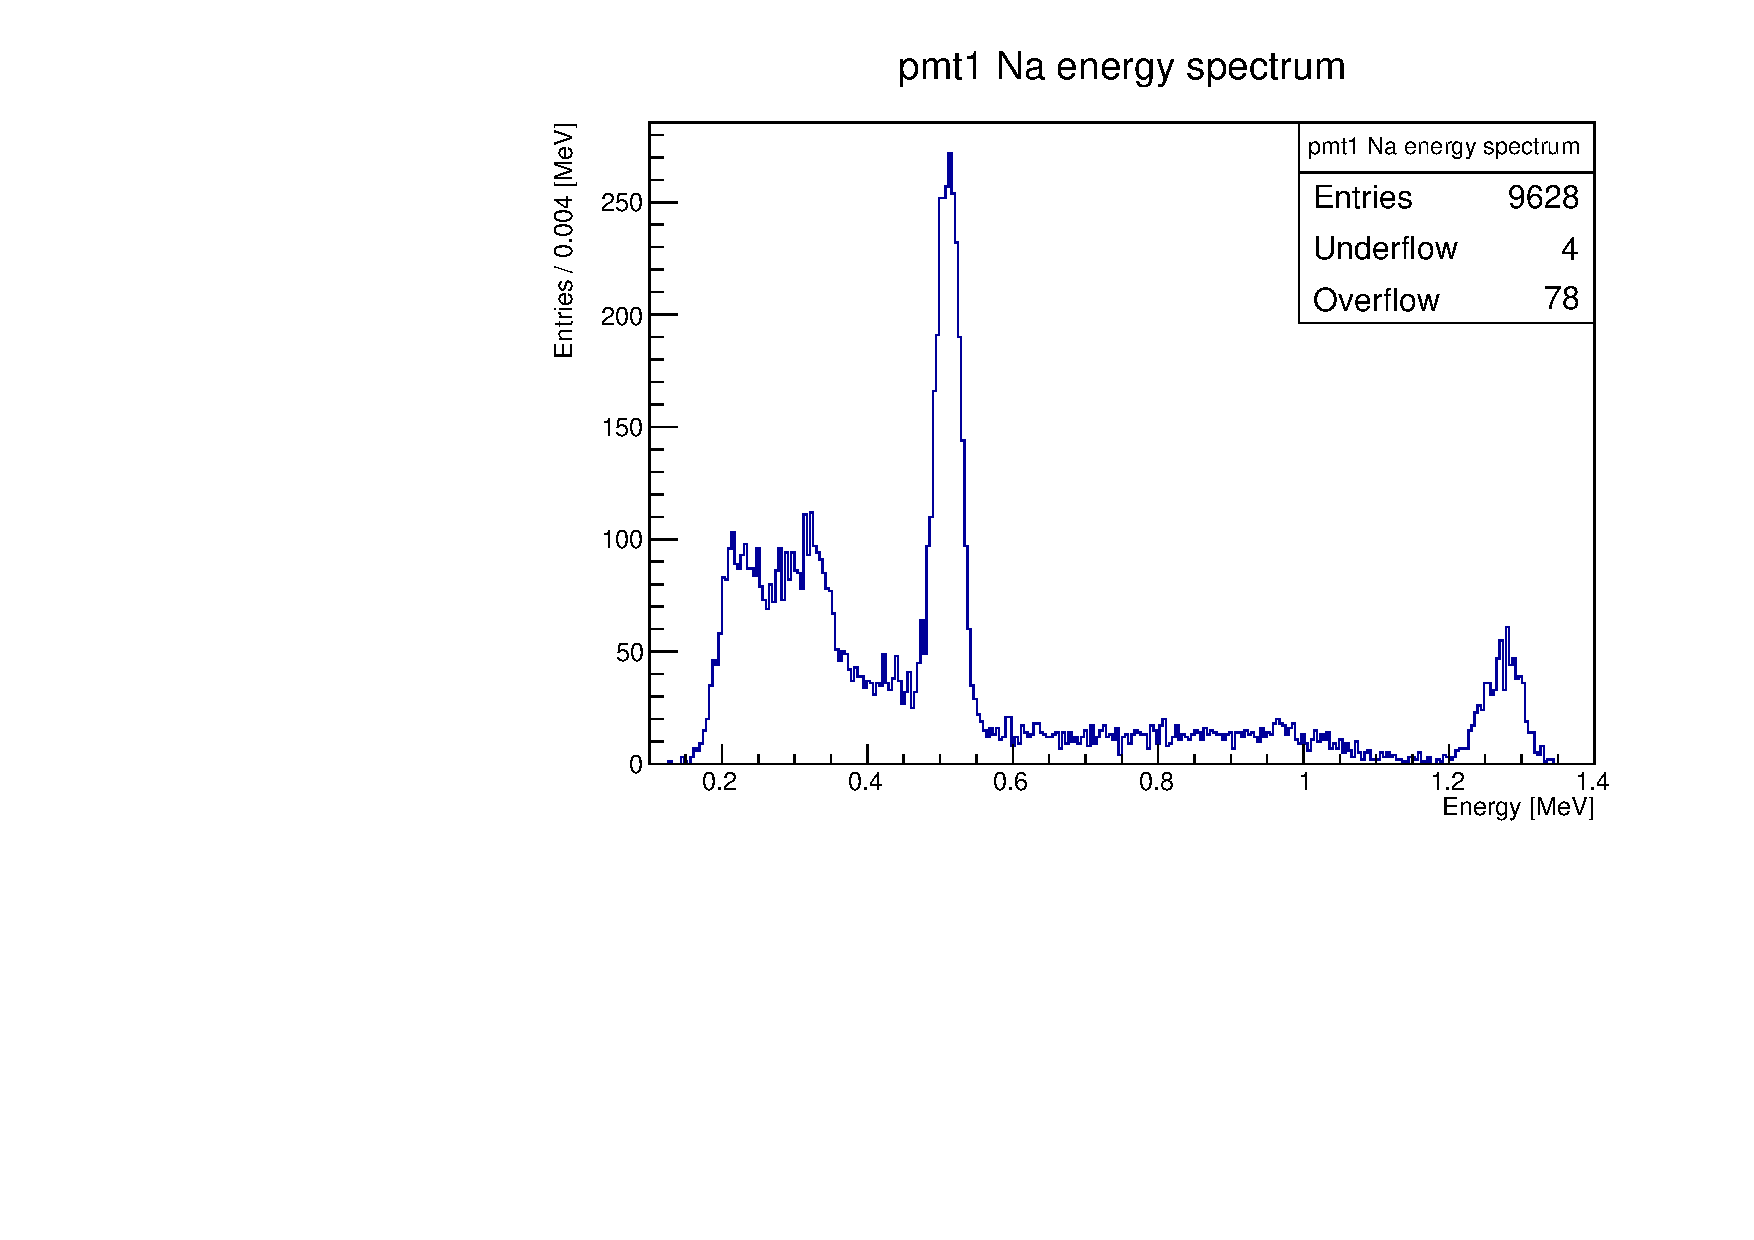
\includegraphics[scale=0.4]{Lab4/Positronio/c1_run8.pdf} 
\caption{$^{22}$Na energy spectrum in mercedes configuration. [06/04/22]}
\label{fig:c1mercedes}
\end{figure}

The distribution of $\Delta t_{123} \equiv \frac{1}{2}(t_1+t_2)-t_3$ is shown in \figurename~\ref{fig:t123distrib_uncut}~\ref{fig:t123distrib_cut}. It is plotted both the whole set of data and the portion of events in which there was also a photon in pmt3. It is clear that there is a correlation in time between the activation of pmt3 and the other 2, as there is a distinct peak near 0 ns. 

\begin{figure}[h!]
\centering
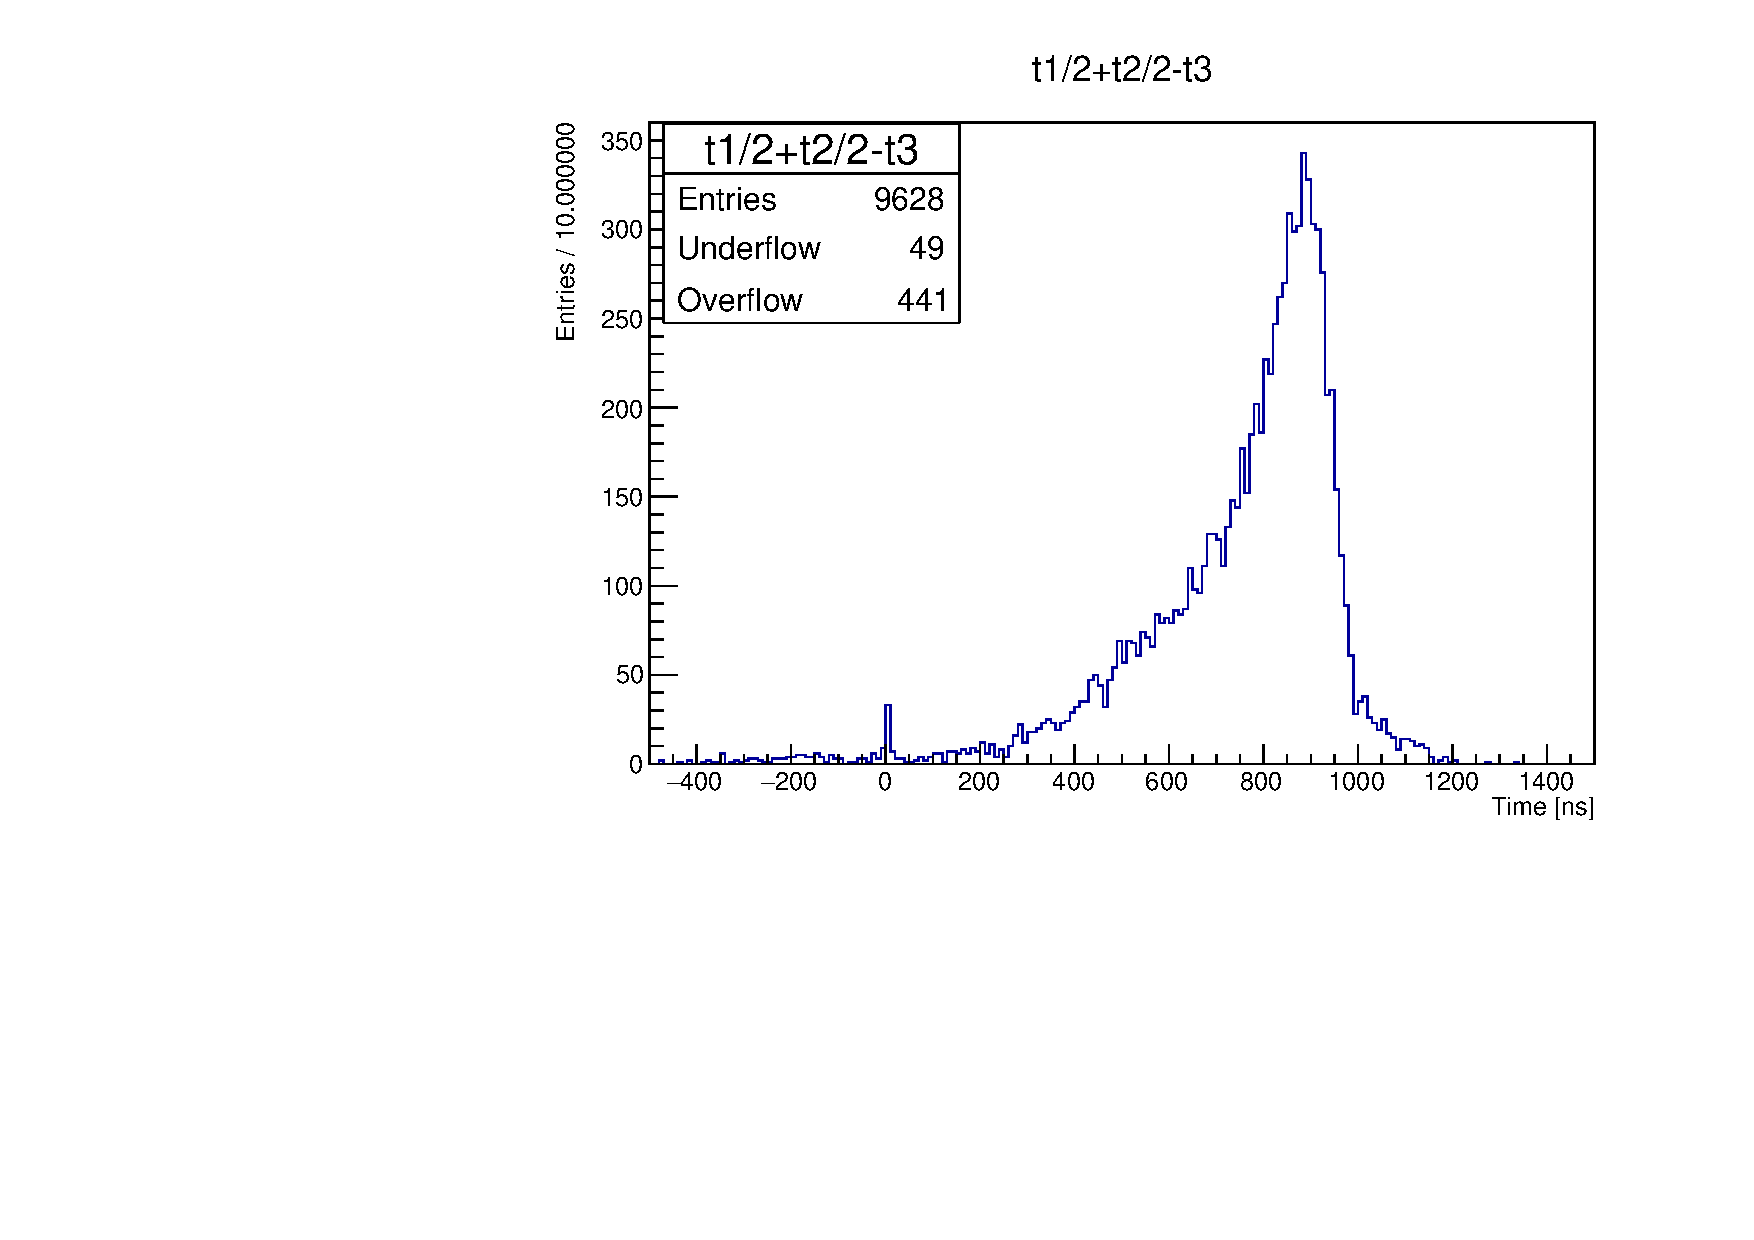
\includegraphics[scale=0.4]{Lab4/Positronio/deltat_uncut.pdf} 
\caption{$\Delta t_{123}$ for the whole set of data. [06/04/22]}
\label{fig:t123distrib_uncut}
\end{figure}

\begin{figure}[h!]
\centering
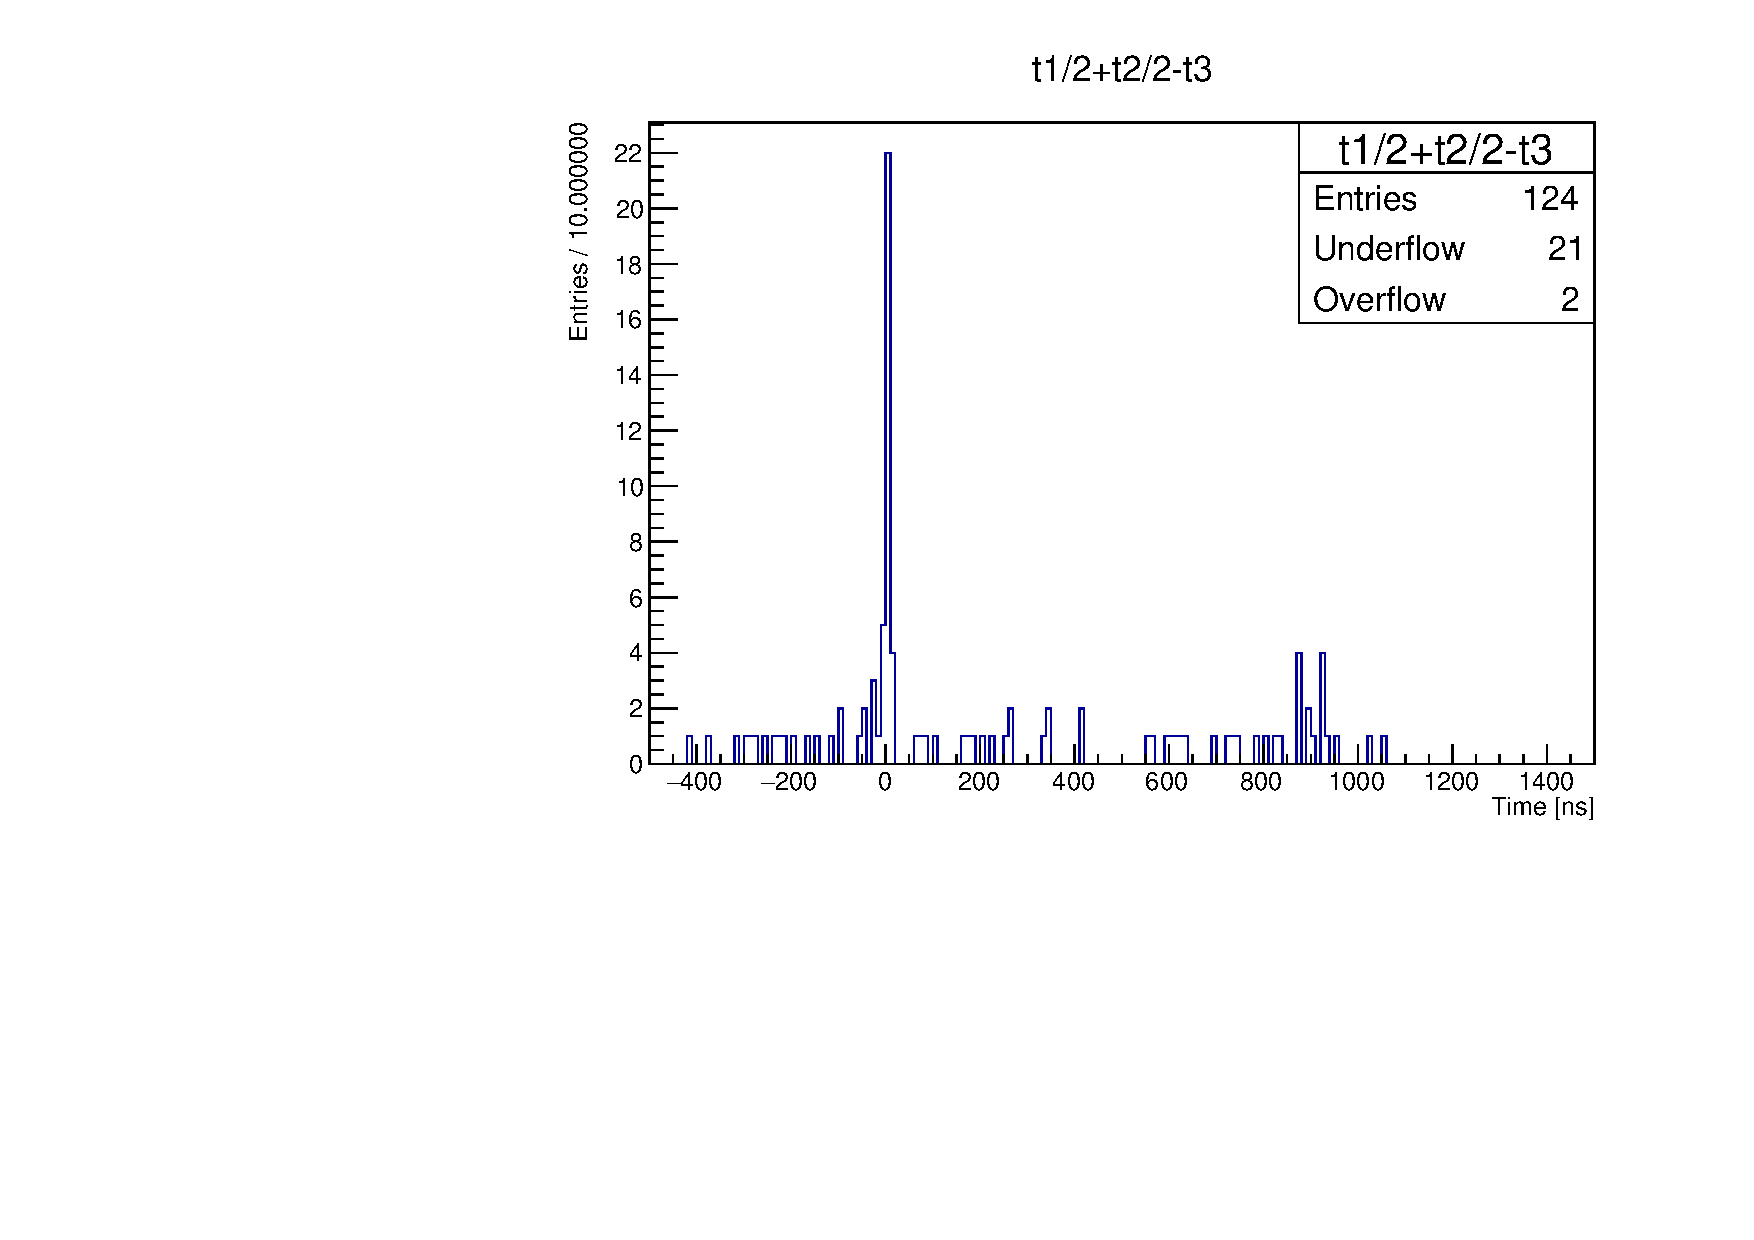
\includegraphics[scale=0.4]{Lab4/Positronio/deltat_cut.pdf} 
\caption{$\Delta t_{123}$ for only the events in which there was also an photon in pmt3. [06/04/22]}
\label{fig:t123distrib_cut}
\end{figure}

\noindent In order to find signal between the noise the following selections were made:

\begin{itemize}
    \item $|t_1-t_2|<13$ ns
    \item $|\Delta t_{123}|<$ 23 ns
    \item $k_1$,$k_2$,$k_3<$ 0.45 MeV
    \item $k_3>0.1$ MeV
\end{itemize}

\noindent where the $t_i$ are the times of the waveforms and $k_i$ the energies of the pulses. 

The cut in time for $t_1$ and $t_2$ was executed upon seeing that the peak of simultaneous pmt 1 and pmt 2 events is about 13 ns wide (\figurename~\ref{fig:t12run8}).

The cut in $\Delta t_{123}$ is to select the events in the peak around 0 ns in \figurename~\ref{fig:t123distrib_cut}

\begin{figure}[h!]
\centering
\includegraphics[scale=0.2]{Lab4/Positronio/t12run8.png} 
\caption{$t_1-t_2$ in ns for run 8 [06/04/22].}
\label{fig:t12run8}
\end{figure}

The cut in energy serves the purpose of cutting away all possible background due to Ne photons, even if of course they can still release less than 0.45 MeV of energy through Compton scattering. It also cuts a good portion of the 511 KeV photons, since 0.45 KeV is under the 511 KeV photopeak, as seen in \figurename~\ref{fig:c1mercedes}. Finally, if in a $3\gamma$ decay one of the photons had energy $>0.45$ MeV, the other two couldn't both be at an angle of less than 140$\degree$ for conservation of 4-momentum ($180\degree - \arccos{\frac{k_1}{2m-k_1}}$). But in the shielded mercedes configuration this makes it almost impossible for such events to be triggered, so the cut on 0.45 MeV reduces the noise, without cutting the possible signal. This is important because for the next section, in which we measure $\alpha_{em}$ from this rate, it is necessary to know if signal has been cut with offline selection and if so how much on average.
\\
\\
In \figurename~\ref{fig:scattersignalvsnoise} the 6 events which make this cut (out of the total 9628) are plotted in red and all other events which fit the same criteria except for $|\Delta t_{123}|>$ 50 ns and not necessarily $k_3>0.1$ MeV are plotted in black. On the x axis is the total energy (k1+k2+k3) corresponding to the event and on the y axis the magnitude of the 3-momentum, assuming the photons are emitted with a perfectly symmetric 120-120-120 degree configuration. 

\begin{figure}[h!]
\centering
\includegraphics[scale=0.3]{Lab4/Positronio/scattersignalvsnoise.png} 
\caption{Signal in time vs not in time. On the x axis is the total energy (k1+k2+k3) in MeV corresponding to the event and on the y axis the magnitude of the 3-momentum in MeV, assuming the photons are emitted with a perfectly symmetric 120-120-120 degree configuration. [06/04/22]}
\label{fig:scattersignalvsnoise}
\end{figure}

\noindent For what had been said until this point, no signal could have been cut out while applying the aforementioned selections. This would lead to the conclusion that the rate is \textit{at most} 6 events per run time. Now this figure suggests something more: not only are all possible signal events triggered contained in those 6 events, but those 6 events are solely made up of signal. All events triggered with the same conditions except time coincidence and minimum $k_3$ belong to a different region on the ($|\Vec{p_{tot}}|,E_{tot}$) plane, in particular at lower energies, except only for three events (the ones nearest to the red points). These three events, like the 6 in red, also have $k_3>0.1$ MeV. But their times are incompatible with actually being a simultaneous $3\gamma$ event. So they could be events that casually happen to fit the criteria, as is expected on such a large sample. How many then of the 6 in time can be expected to be of this casual nature? The frequency of these casual events is about 3 every (2000-50)$\cdot 2 \text{ ns} \rightarrow \simeq 3/4000$ ns. The interval to which the selection has tightened the time coincidence is instead no more than 30 ns wide. This means that about 0.02 casual events can be expected to pass the selection \textit{in time} on a run of this duration. It can then be safely concluded that only signal events coming from $3\gamma$ decays make up those 6 events.

It is interesting to note that the signal events have average total energy of 0.97 MeV, which is 5\% from the expected theoretical value of 1.02 MeV. The discrepancy is too big to be due to energy resolution alone (which is around 3\%), but it can be credited to the fact that photons that don't interact via the photoelectric effect don't release their full energy, for example when Compton scattering, and therefore the total energy can be expected to be less than the maximum achievable in principle. To further investigate this phenomenon it could be fitting to run a Montecarlo simulation. 

Also the momentum magnitude tends to be lower for signal events, as one would expect given that it is calculated to be 0 in the case of a perfectly symmetrical signal event.
\\
\\
Finally the rate of $3\gamma$ events observed with the current configuration is 

\begin{equation}
    R_{3\gamma}= (667 \pm 26)\cdot 10^{-6} \text{ Hz}
\end{equation}



\section{MEASUREMENT OF $\alpha_{em}$}

Since in the last sections the rates of 2$\gamma$ and 3$\gamma$ events have been measured in well defined conditions, taking into account geometrical acceptance and crystal efficiency it is possible to obtain a measurement of $\alpha_{em}$. The ratio between the measured rates is

\begin{equation}
\label{ratetoalpha}
\begin{split}
    \frac{R_{3 \gamma}}{R_{2\gamma}} & =\frac{R_{\beta^+} \int_{geom}{\varepsilon(k_1) \varepsilon(k_2)\varepsilon(k_3) d\sigma_{3\gamma}}}{R_{\beta^+} \int_{geom}{\varepsilon(k_1) \varepsilon(k_2) d\sigma_{2\gamma}}}\\
    & =\frac{\int_{geom}{\varepsilon(k_1) \varepsilon(k_2)\varepsilon(k_3) d\sigma_{3\gamma}}}{\varepsilon^2(m)\int_{geom}{d\sigma_{2\gamma}}}
    \end{split}
\end{equation}

\noindent where the integral is performed over the region of phase space in which the photons are detected by the pmt configuration, which was taken to be the mercedes one in \figurename~\ref{fig:mercedes} for $3\gamma$ and the one in \figurename~\ref{fig:e6config} for $2\gamma$.  $d\sigma$ is the differential cross section in that point of phase space, $R_{\beta^+}$ is the emission rate of $e^+$ by the $^{22}$Na source and $\varepsilon(k)$ is the NaI crystal's intrinsic detection efficiency for photons of energy $k$. In the following calculations the cross sections will be evaluated in the non relativistic limit, since we know that the $e^+$ and $e^-$ annihilate almost at rest in the lab frame (see Section 3). Also, all quantities will be expressed in natural units ($\hbar=c=1$).


\\
\\
The rates $R$ are easily obtained by counting the required events in a run and dividing by its duration, which can be precisely measured using the \texttt{Trigger Time Tag} feature of the ADC's waveform recording software \texttt{wavedump}. $R_{3\gamma}$ is taken from the previous Section while $R_{2\gamma}$ is taken by triggering in logic OR combination for the two pmts. Its value is $331 \pm 18$ Hz. The initial rate $R_{\beta^+}$ cancels out so the most challenging part is evaluating the two integrals that remain and the efficiencies.
\\
\\
Since the $\gamma \gamma$ decay is monochromatic in the lab frame and the photons are always back to back, the only important variable is the direction (specified by two angles) along which the two $\gamma$ propagate. Furthermore, the differential cross section is constant in said direction

\begin{equation}
    \frac{d\sigma_{2\gamma}}{d\Omega}=\frac{\alpha_{em}^2}{vm^2}
\end{equation}

\noindent where $v$ is the velocity of the incoming $e^+$ (if we take $e^-$ to be still) and $m$ its mass. Then the integral is simply

\begin{equation}
\label{\sigma2gamma}
     \int_{geom}{d\sigma_{2\gamma}}=\frac{d\sigma_{2\gamma}}{d\Omega}2\Omega^{far}_{2\gamma}
\end{equation}

\noindent where $\Omega^{far}_{2\gamma}$ is the solid angle of the farthest of the two pmts (the most stringent condition of the two).
\\
\\
The $3\gamma$ integral is more complicated. The fact that the final state has now \textit{three} bodies means that the differential cross section can in principle depend on 9-4=5 parameters instead of 2 as it did for $2\gamma$. Fortunately in the case of $d\sigma_{3\gamma}$ the only dependence is from two parameters, which can be chosen in different ways according to preference. For example Landau-Lifshitz ["\textit{Course of Theoretical Physics Vol. 4, Quantum Electrodynamics }"] give $d\sigma_{3\gamma}$ in terms of the energies of two of the photons


\begin{equation}
    d\sigma_{3\gamma}=\frac{1}{6}\frac{8\alpha_{em}^3}{vm^2} F(k_1,k_2)dk_1 dk_2
\end{equation}

with 
\begin{equation*}
    F(k_1,k_2)=\left[\left(\frac{m-k_3}{k_1k_2} \right)^2 + \left(\frac{m-k_2}{k_1k_3} \right)^2 + \left(\frac{m-k_1}{k_2k_3} \right)^2\right]
\end{equation*}


\noindent where $k_3=2m-k_1-k_2$.

\noindent For the purposes of this work it is best to express the cross section in terms of the angles between one photon (say, $k_1$) and the other two ($\theta_2$ and $\theta_3$ with $k_2$ and $k_3$ respectively). To do so it first is necessary to express $k_1$ and $k_2$ in terms of $\theta_2$ and $\theta_3$. After some calculation one obtains

\begin{equation}
    k_1=\frac{2m}{1-\frac{s_2+s_3}{s_2c_3+s_3c_2}}
\end{equation}

and 

\begin{equation}
    k_2=\frac{2m}{1+\frac{s_2}{s_3}(1-c_3)-c_2}
\end{equation}

\noindent where $s_i$ and $c_i$ stand for $sin\theta_i$ and $cos\theta_i$. As expected the expression for $k_1$ is symmetric in the two angles while the one for $k_2$ is different.

\noindent To change variables it's sufficient to insert the absolute value of the Jacobian

\begin{equation}
    dk_1dk_2=|J|d\theta_2d\theta_3
\end{equation}

where

\begin{equation}
     J= \begin{vmatrix} \dfrac{\partial k_1}{\partial \theta_2} & \dfrac{\partial k_1}{\partial \theta_3} \\[2ex] \dfrac{\partial k_2}{\partial \theta_2} & \dfrac{\partial k_2}{\partial \theta_3} \end{vmatrix}
\end{equation}
  
\noindent This is equal to

\begin{equation*}
     J= \frac{4m^2s_2s_3}{[s_2(1-c_3)+s_3(1-c_2)]^4}(1-(c_2c_3-s_2s_3)^2)
\end{equation*}

  

\noindent In conclusion then 


\begin{equation}
    d\sigma_{3\gamma}=\frac{4\alpha_{em}^3}{3vm^2} F(k_1(\theta_2,\theta_3),k_2(\theta_2,\theta_3))|J|d\theta_2d\theta_3
\end{equation}
\\
\\
In the present case the pmts have finite dimension, so the possible angles between the accepted photons can vary a little from 120 degrees. For this reason to simplify calculations one can assume the differential cross section to be constant to the first order, and in particular equal to its value in the 120-120-120 case, and then multiply it by the small interval in which $\theta_2$ and $\theta_3$ can vary and still be detected.

\noindent With this approximation

\begin{equation}
    d\sigma_{3\gamma}\simeq \frac{\alpha_{em}^3}{3vm^2} d\theta_2d\theta_3
\end{equation}
\\
\\
Substituting the differential cross sections found into (\ref{ratetoalpha}), considering the fraction of phase space occupied by the detectors' geometry \footnote{First the solid angles in which a reference photon, e.g. $k_1$, would hit the 3 pmts are evaluated. Then the angle along which the plane containing the other two photons spins is considered, and the fraction of such angle in which the plane contains the other two pmts is taken into account.} and multiplying by the wiggle room of $\theta_2$ and $\theta_3$, one gets, with a few approximations,


\begin{equation}
    \alpha_{em}=\frac{12\pi^2(1-\cos{\rho})\varepsilon^2(m)}{\varphi^3\Tilde{\varphi}(2\varphi+\Tilde{\varphi})\varepsilon^3(2m/3)}\frac{R_{3\gamma}}{R_{2\gamma}}
\end{equation}

where $\rho$ is the half of the angle occupied by the surface of pmts 1 and 2 (which are $\simeq$ equidistant) as seen from the center in configuration E6 and $\varphi$ and $\Tilde{\varphi}$ are the same ($\Tilde{\varphi}$ for pmt3) in configuration C6.
\\
\\
The only thing left to evaluate are the efficiencies. $\varepsilon(m)$ is easier to evaluate since it can be measured directly from the data from which $R_{2\gamma}$ is measured. It is sufficient to consider a run triggered on the logic OR of the two pmts and measure the probability that if one pmt is activated the other is too and vice versa. With this method the efficiencies come out to be\footnote{The uncertainties have been evaluated like specified for the $P$ in Section 3}

\begin{equation}
    \varepsilon_1= 0.254\pm 0.001 \quad \quad \quad \varepsilon_2= 0.329\pm 0.001
\end{equation}

\noindent One problem with this approach is that since pmt2 is closer not all photons that hit it are supposed to hit pmt1. Since the number of photons that hit the pmts follow the inverse square law, it would be reasonable to expect that

\begin{equation}
    \frac{\varepsilon_1}{\varepsilon_2} \simeq \frac{d_2^2}{d_1^2}
\end{equation}

substituting

$$0.77 \simeq 0.85$$

which is true to 10 \%.
\\
\\
The real problem however are the $\varepsilon(2m/3)$. Although no conclusive data was found on the subject, various sources from literature suggest that the intrinsic efficiency can vary even by a factor of 100\% between 510 KeV and 330 KeV, usually being greater at 330 KeV. However, we are not capable of giving a satisfactory estimate of $\varepsilon(2m/3)$ with the data at our disposal. For this reason the same efficiency as the one for $k=m$ will be used in the following calculation, keeping in mind that and eventual factor of difference would appear to the \textit{third power} in the expression for $\alpha_{em}$.
\\
\\
Finally, with these hypotheses, the value for $\alpha_{em}$ is

\begin{equation}
    \alpha_{em}=  0.2990 \pm   0.0001
\end{equation}

Not only is this value not compatible with the PDG value $7.3 \cdot 10^{-3}$, but its uncertainty has been calculated only from statistical dependence upon the $R$. The systematic error on this measurement is much greater, both because of the geometrical approximations we applied in integrating the differential cross section, both because of the unknown value of $\varepsilon(2m/3)$, which appears to the third power in the final expression.
\section{TIME RESOLUTION}
In this section the objective is to measure the time resolution of our system. The algorithm used to determine the time at which a waveform's event took place given the waveform is described in \appendixname~\ref{appendix:t_algorithm}. For example by triggering on the coincidence of two pmts and plotting their $\Delta t_{12}\equiv t_1-t_2$ it is possible to determine the resolution of the system (\figurename~\ref{fig:t12}).

\begin{figure}[h!]
\centering
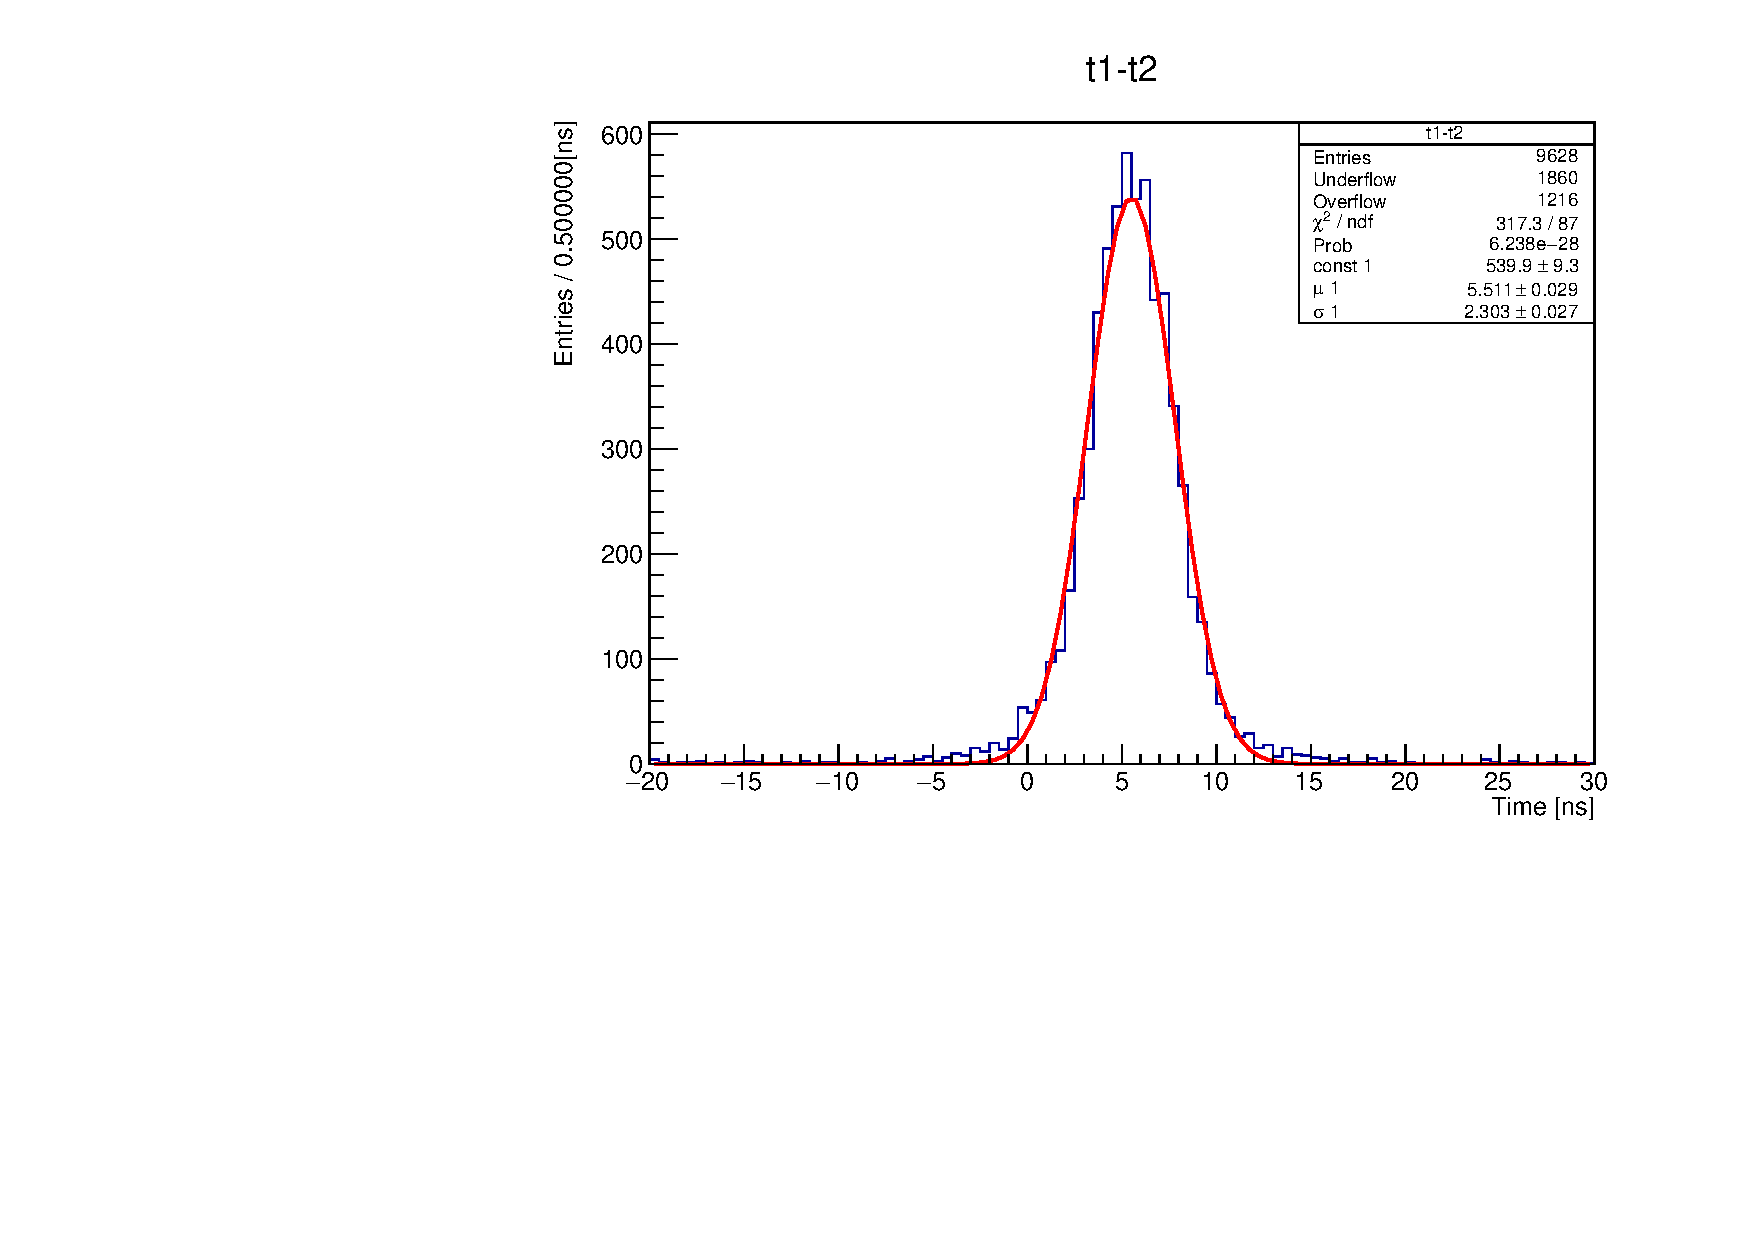
\includegraphics[scale=0.35]{Lab4/Positronio/t12_gaus_run8.pdf} 
\caption{Difference between the time triggered by pmt1 and pmt2. [06/04/22]}
\label{fig:t12}
\end{figure}


\\
\\
As seen in following Figures, the resolution in about 2.2-2.3 ns. This is acceptable considering the fact that the ADC's time resolution is 4 ns.

Also the average of these $\Delta t_{12}$ distribution is different from zero (a few ns often) even for events that physically should be instantaneous on the ns scale. The non null average could be due to the fact that while passing through the various NIM modules and finally arriving at the ADC the two pmt signals travel trough different channels with different wires. If some of these components have slightly different delays because of manufacturing imperfections, this could lead to effect observed. However, this hypothesis has been tested by switching the connections between the pmts and the whole following circuit. Nonetheless similar results for $\Delta t_{12}$ are found (\figurename~\ref{fig:invertedt12}).
Therefore, we have only two alternative hypotheses. One is that this effect depends on the wiring of the pmts to the NIM rack, which was not done by our group and could be different between the two. Another possible explanation is that the two detectors themselves have different response times. 

\begin{figure}[h!]
\centering
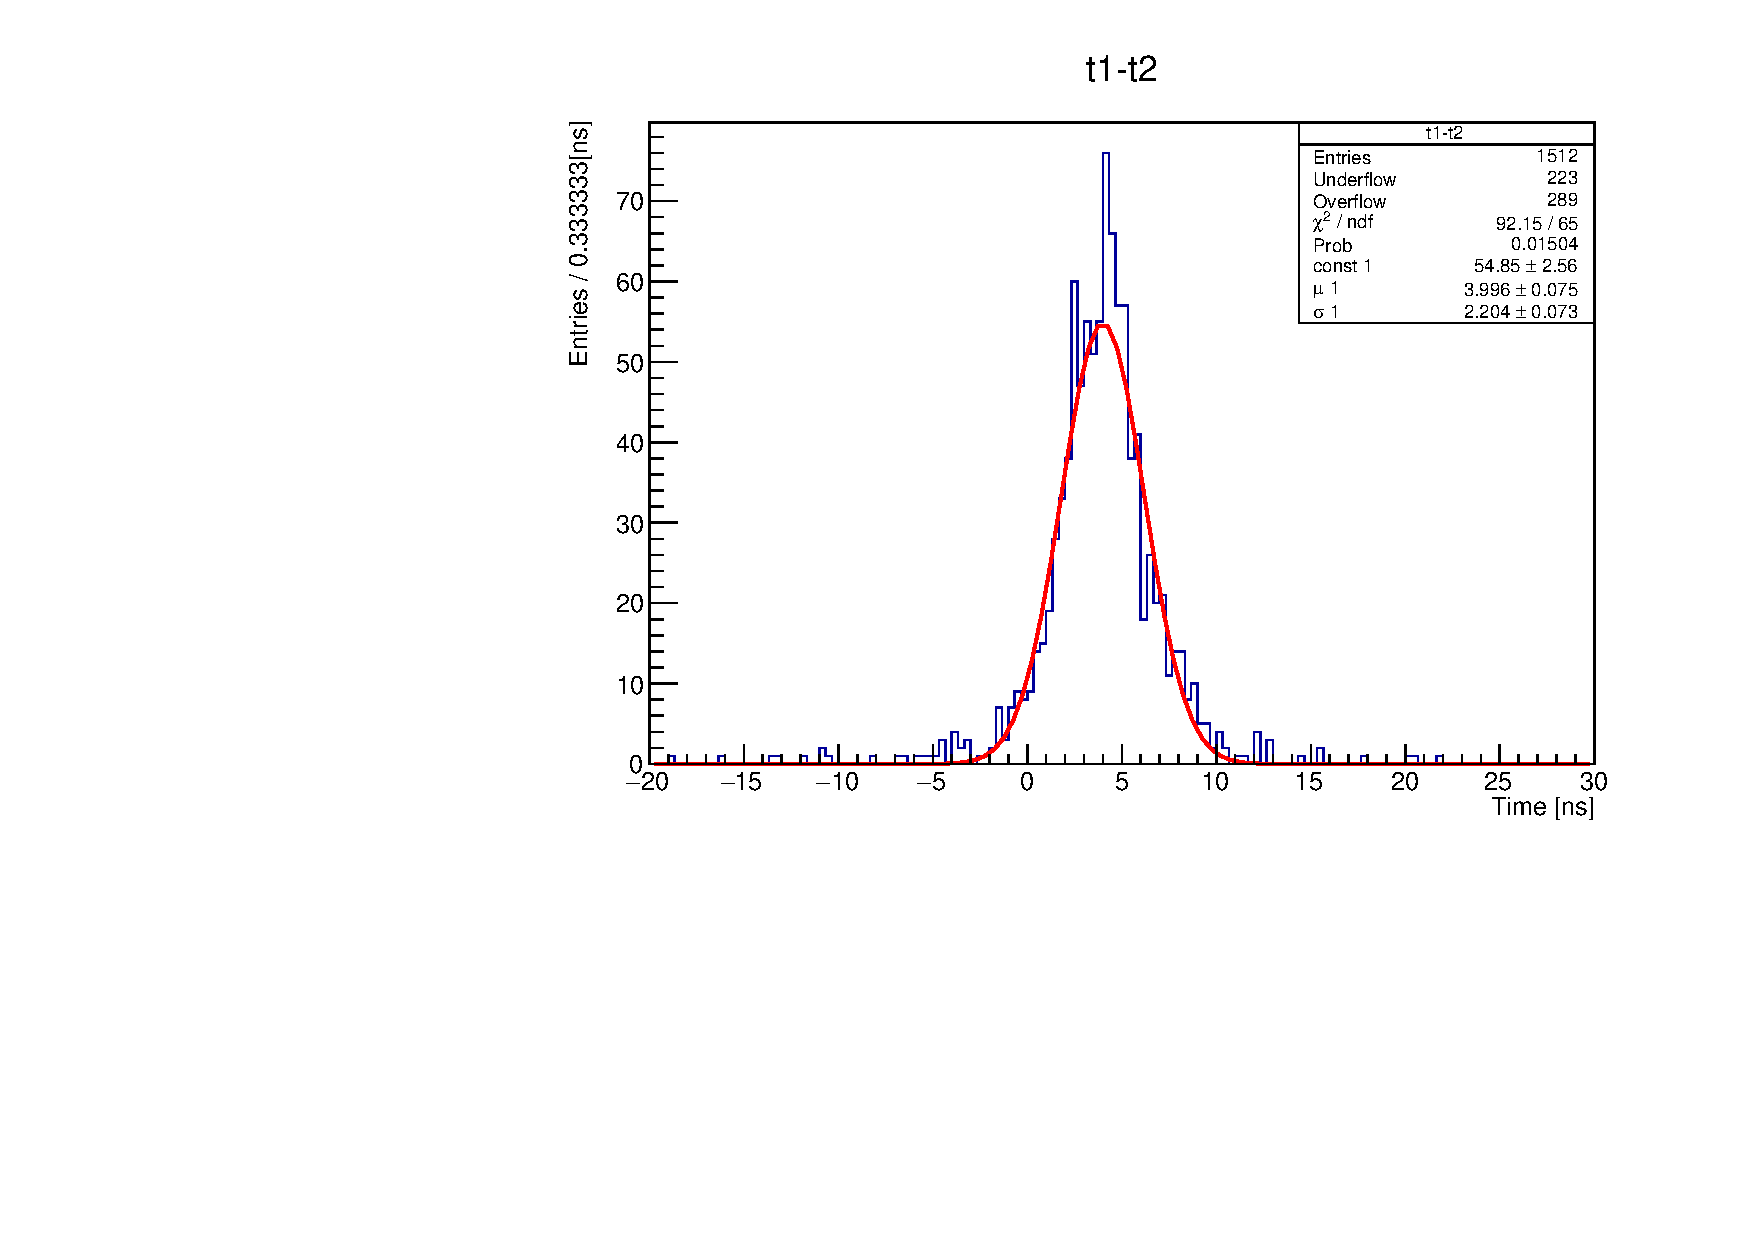
\includegraphics[scale=0.35]{Lab4/Positronio/t12_gaus_run7.pdf} 
\caption{Difference between the time triggered by pmt1 and pmt2 when switching the connections. [05/04/22]}
\label{fig:invertedt12}
\end{figure}



\section{SEARCH FOR NON NULL LIFETIME STATE}

Having developed an algorithm to evaluate the time at which the events take place with respect to each other with a resolution of about 2 ns, it is possible to exploit the presence of the simultaneous (on the scale of our resolution) Ne photon (\figurename~\ref{fig:22na}) to find possible states formed by $e^+$ with a life time of the order of our resolution or greater. This would be orthopositronium, whose lifetime \textit{in vacuum} is about 140 ns. 

In order to do so the pmts were arranged in the "T" configuration shown in \figurename~\ref{fig:TconfigL1} (source in L1) and \figurename~\ref{fig:TconfigI2} (source in I2). The objective is to search through $2\gamma$ events, easily detected with pmt1 and pmt2 at 180 degrees, and study the distribution of the time after which photons with energy greater than 0.6 MeV (so that they are surely Ne photons) hit pmt3. 



\noindent In \figurename~\ref{fig:t123Tempty} the distribution of $\Delta t_{123}$ (as defined in previous sections) for \figurename~\ref{fig:TconfigL1} is shown. The same is done for the configuration in which the source is shielded by iron slabs surrounding the source cell as in the image and in the case of aerogel, instead of iron, in the same cells. These are reported in \figurename~\ref{fig:t123Tiron} and \figurename~\ref{fig:t123Taero} respectively. In all of these cases the distribution is not symmetrical and, in fact, if one attempts to fit these curves with a gaussian, it is evident that there is a tail to the right that dies off less rapidly than a gaussian tail would. This could be a sign that positrons emitted by the source also form states that subsequently decay in at least two photons and whose lifetime is noticeable with respect to the resolution of this apparatus. To find out the mean lifetime of this supposed state, a fit of the former distributions was made with a gaussian+exponential model instead of a simple gaussian. The mean lifetime for each material are shown below:
\begin{itemize}
    \item $\tau_{air}=2.5 \pm 0.2$ ns
    \item $\tau_{iron}= 3.0 \pm 0.6$ ns
    \item $\tau_{aerogel}= 3.4 \pm 0.6$ ns
\end{itemize}

\begin{figure}[h!]
\centering
\includegraphics[scale=0.15]{Lab4/Positronio/MicrosoftTeams-image(1).png} 
\caption{Configuration in which the source is placed in L1 (not shielded). [23/03/22]}
\label{fig:TconfigL1}
\end{figure}

\begin{figure}[h!]
\centering
\includegraphics[scale=0.15]{Lab4/Positronio/MicrosoftTeams-image(3).png} 
\caption{Configuration in which the source is placed in I2 (surrounded by iron or aerogel). [07/04/22]}
\label{fig:TconfigI2}
\end{figure}

\begin{figure}[h!]
\centering
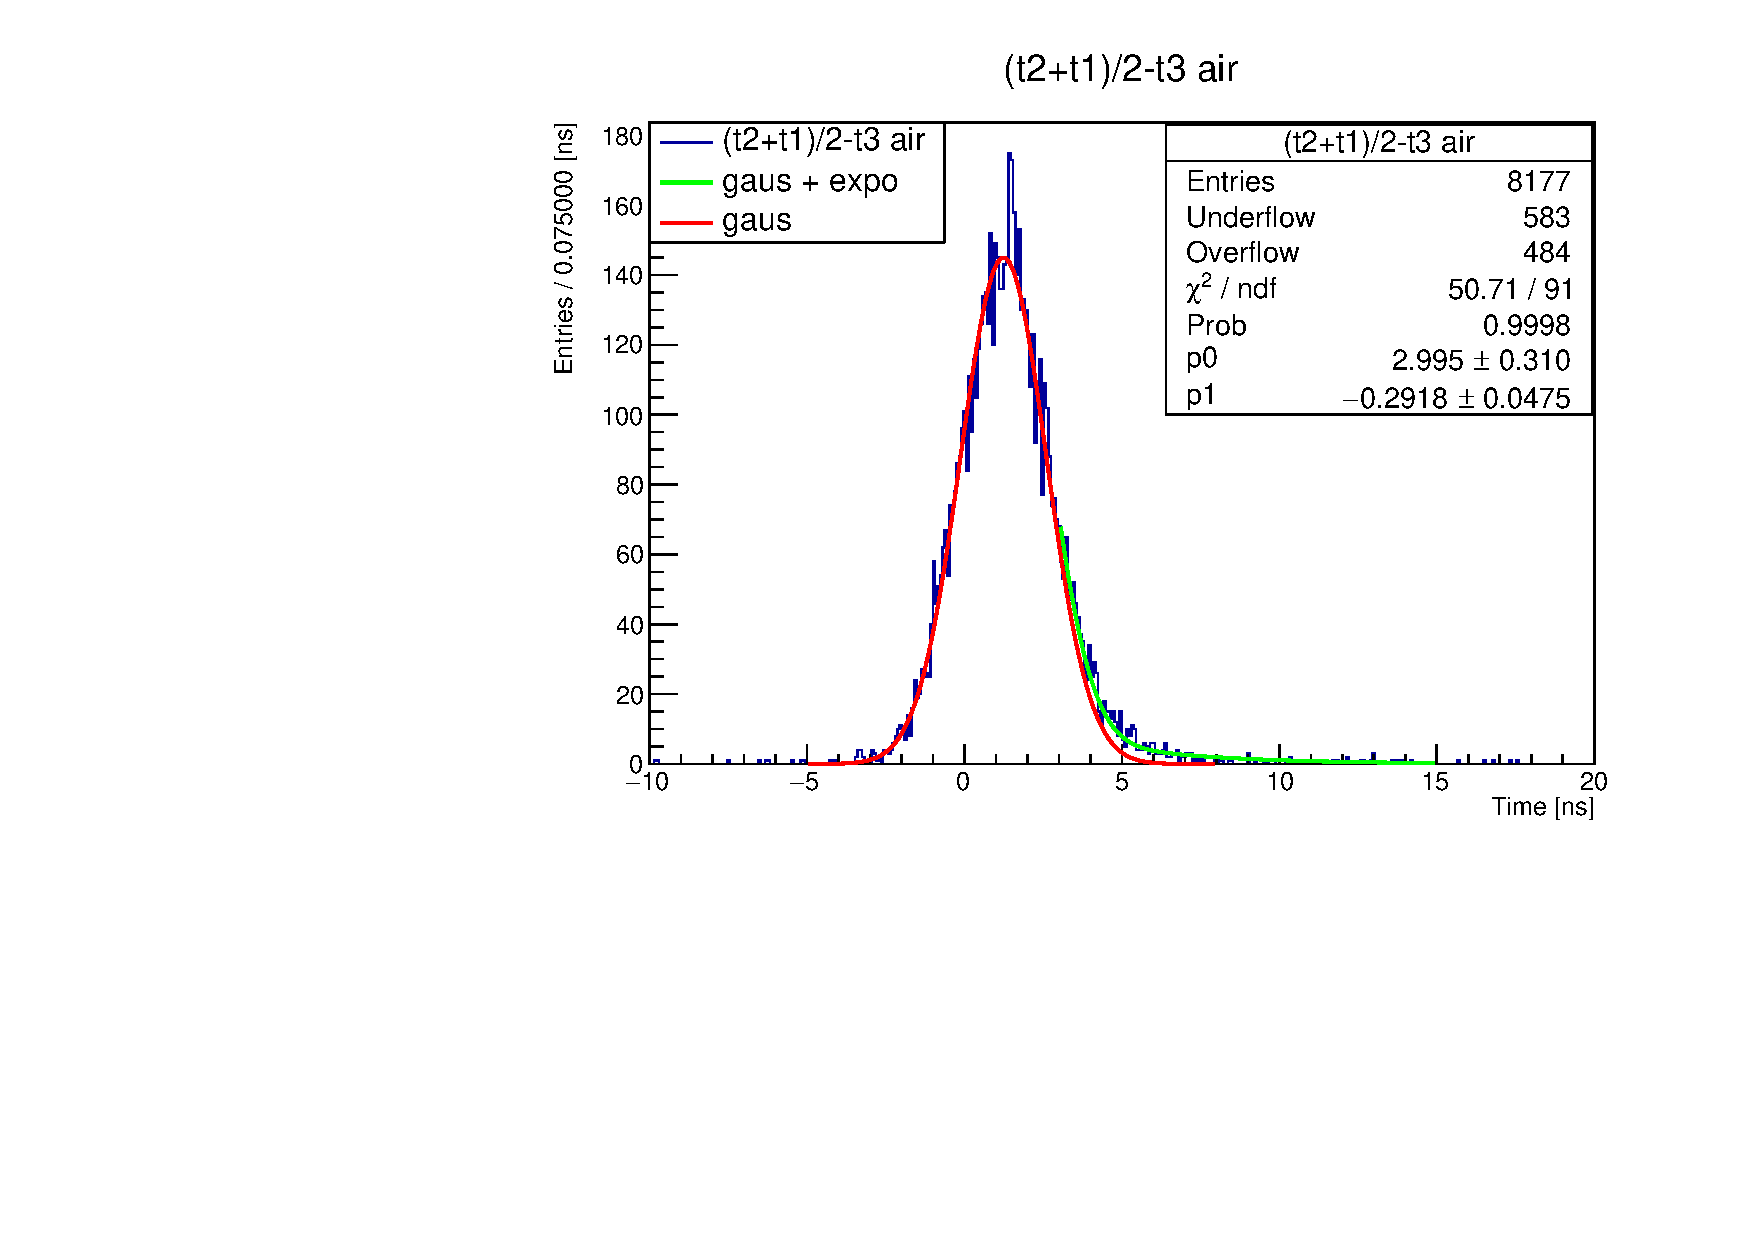
\includegraphics[scale=0.45]{Lab4/Positronio/life_air.pdf} 
\caption{$\Delta t_{123}$ distribution without any materials. [24/03/22]}
\label{fig:t123Tempty}
\end{figure}


\begin{figure}[h!]
\centering
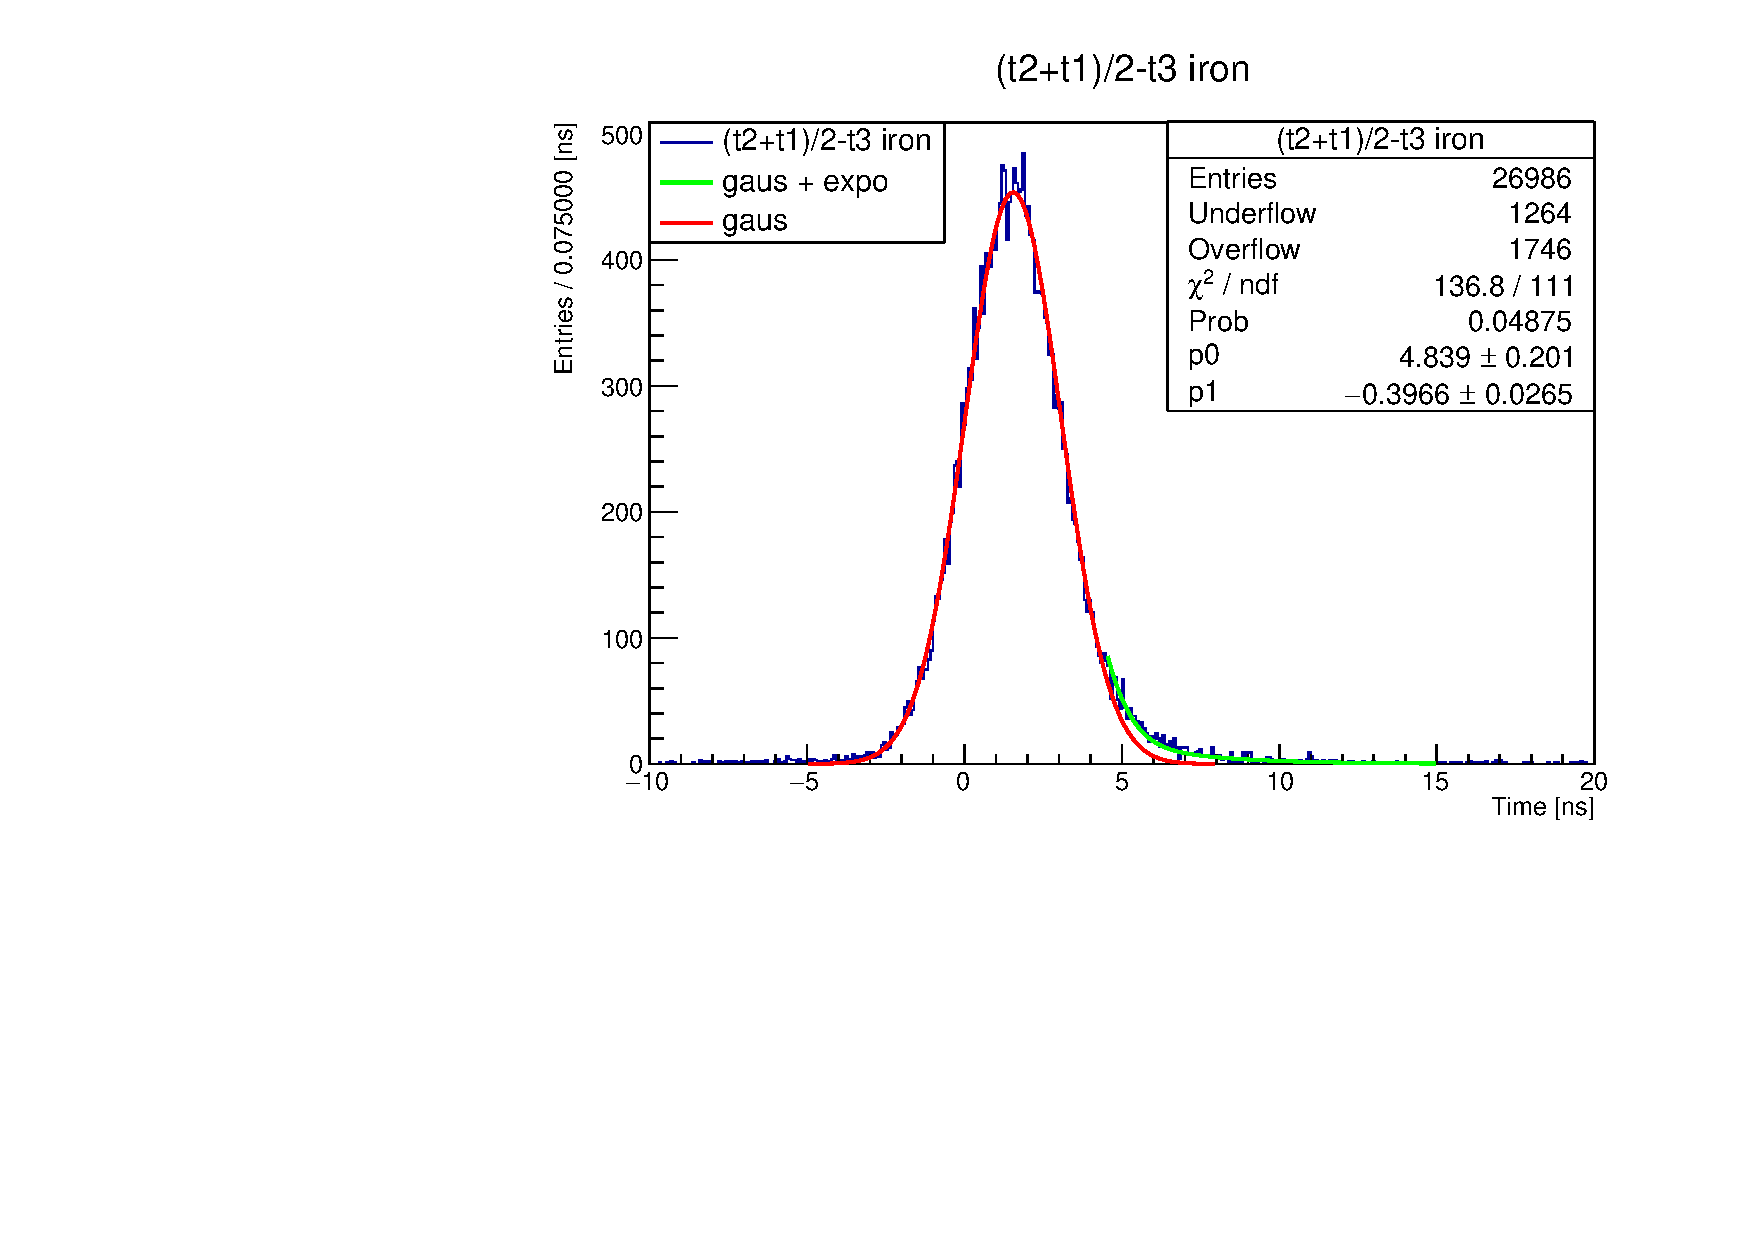
\includegraphics[scale=0.45]{Lab4/Positronio/life_iron.pdf} 
\caption{$\Delta t_{123}$ distribution in iron. [07/04/22]}
\label{fig:t123Tiron}
\end{figure}


\begin{figure}[h!]
\centering
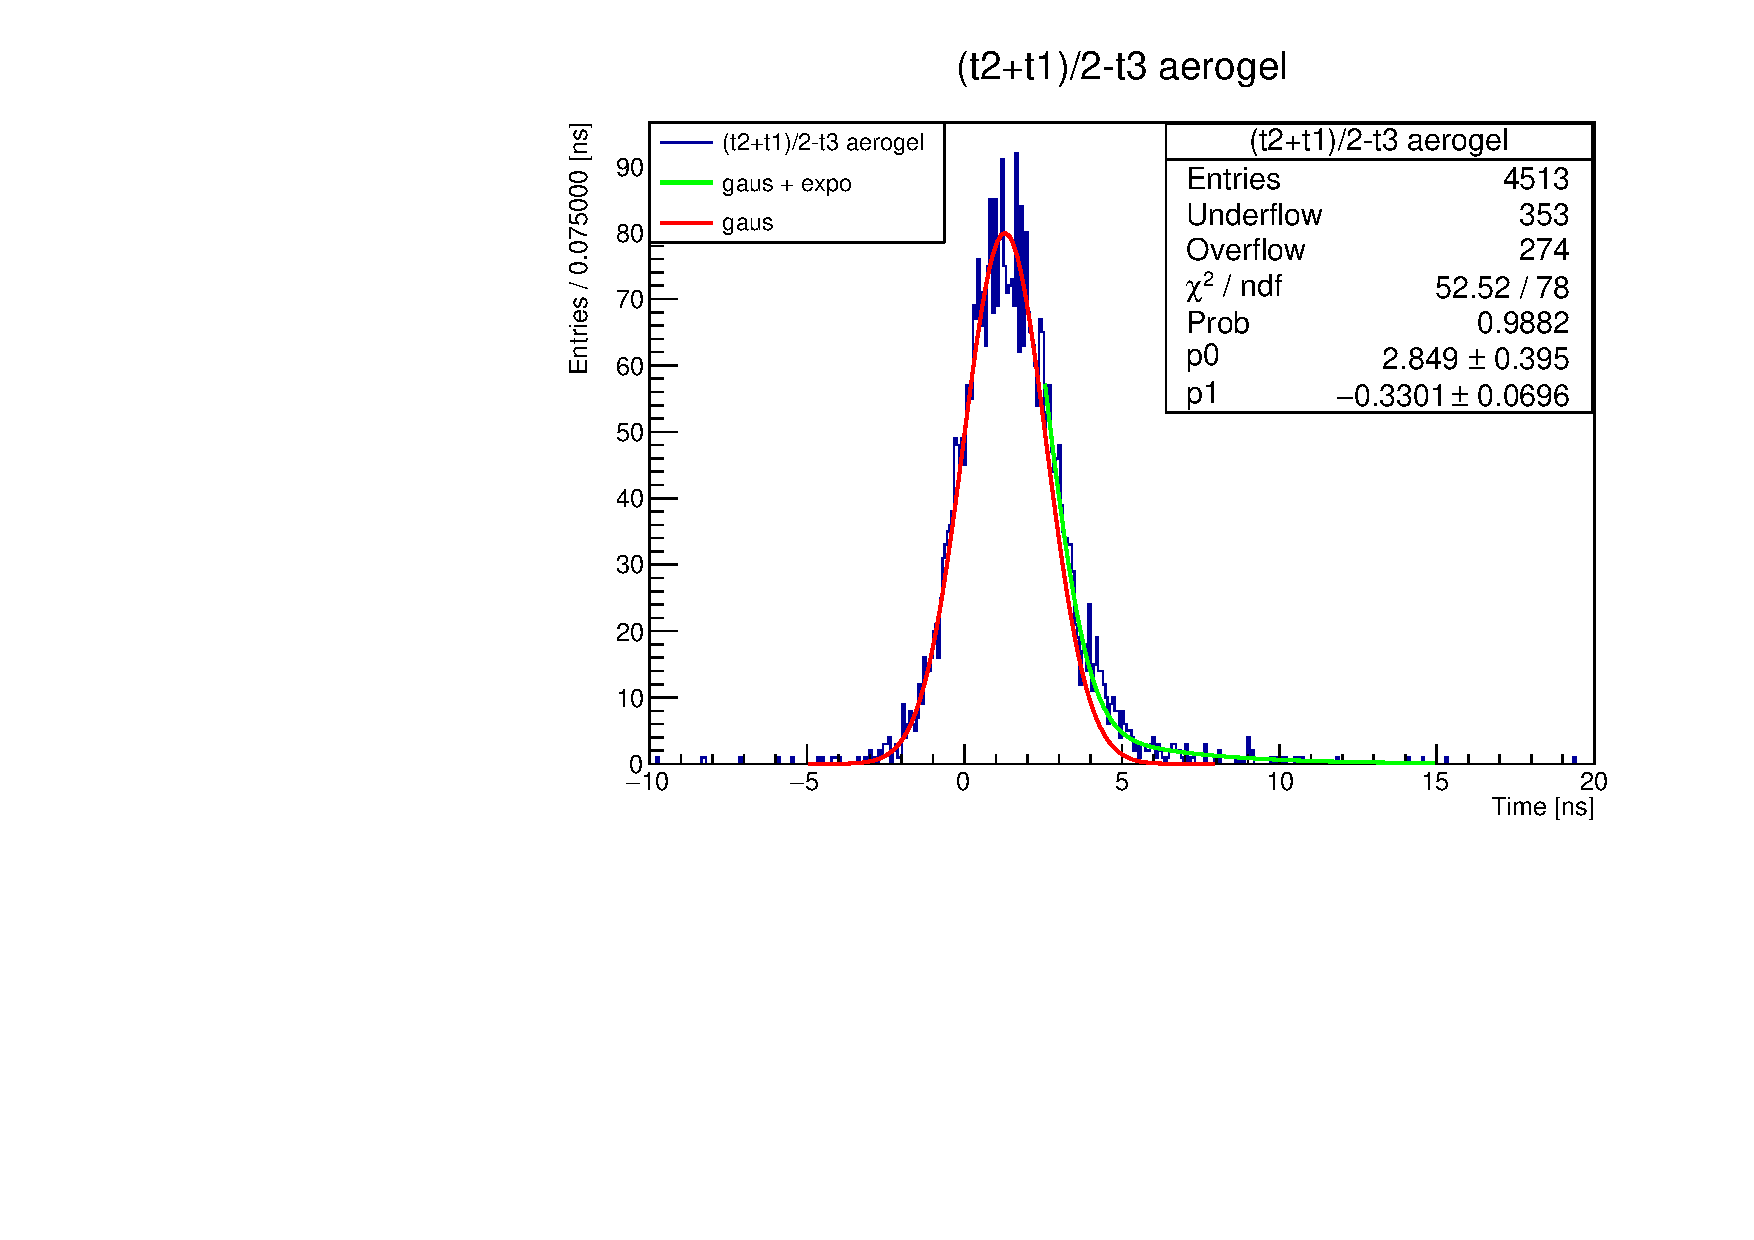
\includegraphics[scale=0.45]{Lab4/Positronio/life_aerogel.pdf} 
\caption{$\Delta t_{123}$ distribution in aerogel. [07/04/22]}
\label{fig:t123Taero}
\end{figure}


\\
\\
Even if different materials were used, with different density and porosity (porosity in aerogel is typically between 90 to 99\%), the lifetimes are compatible. Our hypothesis is that what is being observed is actually the mean lifetime of such state in the \textit{plastic} that constitutes the grid. For the purposes of this work the grid couldn't be removed, and it could have the potential of slowing down the $e^+$ to energies where they could form bound states. Using the data from ["\textit{Stopping Powers and Ranges of Electrons and Positrons}", NBSIR 82-2550] it can be deduced that in a plastic material the expected CDSA range for a $e^+$ of 545 KeV is around 1.6-1.7 millimeters (in water around 2mm and in aluminum around 1mm). Because the plastic in such grid was no less than 2mm thick it is reasonable to assume that the positrons were stopped before even reaching the adjacent cells, thus explaining why the lifetimes were compatible in all three cases. 

Given the situation, it is adequate to combine these measures to obtain the mean lifetime of this state in the plastic that constitutes the grid

\begin{equation}
    \tau= 2.6 \pm  0.2 \; \text{ ns}
\end{equation}





\section*{DECLARATION OF AUTHENTICITY}
The authors of this work declare that its contents are original and the fruit of their work alone.

\clearpage
\begin{appendices}
\section{Charge and amplitude algorithms}\label{appendix:c_a_algorithm}
The first step to obtain an estimate of the charge released in the photomultiplier is to compute the baseline of the waveform. This is done by taking the average value in the first 80 ns where the signal is expected to be flat. In case a pulse is present in this range, in order to avoid an erroneous result, the event is discarded. Next, the charge is computed as the sum of the differences between the baseline and the value of the signal in the range [1.2 $\mu s$, 3.8 $\mu s$] starting from the beginning of the acquisition. This interval was chosen since it prevents from considering signals that are only partially sampled but still be large enough to contain the whole waveform. 

The amplitude is instead computed as the maximum difference between the baseline and the value of the waveform in the range mentioned before.

\section{Time algorithm}\label{appendix:t_algorithm}
The time associated with each event is the estimate of the instant (in range [1.2 $\mu s$, 3.8 $\mu s$]) at which the signal, during its descent, crosses the middle point between the baseline (see \appendixname~\ref{appendix:c_a_algorithm}) and the minimum value of the waveform. To do so, the bin closest to the instant mentioned above is found and, in order to obtain a continuous range of possible values for $t$, a linear fit of the five bins around it is performed. The intersection between the linear best fit curve and the halfway point between the baseline and the minimum is what is taken to be $t$.

\section{$N_{12}$ and $N^{rdm}_{12}$ UNCERTAINTIES}\label{appendix:N_uncertainties}


For $N_{12}$ the maximum likelihood estimator of a Poissonian distribution is the average of the values recorded and since there is only one measurement available, the estimator coincides with $N_{12}$ itself. In the case of the Poissonian distribution this estimator is also the sufficient statistic from Darmois Theorem and therefore it fits Cramer-Rao's criteria for minimum variance bound.

Then, as an estimator $N_{12}$'s, distribution is the Poissonian itself. Its variance is therefore equal to the expected value of its distribution, which again is unknown. Consequently $N_{12}$ is used to estimate its own variance: the number reported is $N_{12} \pm \sqrt{N_{12}}$. 

For $N_{12}^{rdm}$ the situation is different, since it isn't an actual counting of events. It too is an estimator of the expected value (in this case of the poissonian distribution of random coincidences), but now its distribution is \textit{not} the poissonian itself. In fact, aside from constants, it is proportional to the product of the number of events in the respective photopeaks recorded $N_1$ and $N_2$ (from which $f_1$ and $f_2$ were derived). So it is the product of two poissonian distributions. Its variance and possible unbiasedness must then be determined from \ref{eqn:N12rdm}. In doing so it must also be taken into account that the two quantities $N_1$ and $N_2$ are in fact \textit{correlated}. In this case the correlation was ignored in determining the uncertainty because its effect to is negligible compared to the fact that the two $N$ are extremely different in any case.  


\section{Instrumentation}\label{appendix:strumentation}

\begin{itemize}
\item Radioactive calibration sources $^{60}$Co, $^{137}$Cs and $^{22}$Na
\item 3 NaI crystals
\item 3 photomultiplier Tubes (PMT) 
 \item NIM module: ADC N6725S and CAEN waveform acquisition software "\textit{wavedump}" 
\item NIM module: Discriminator unit (4 CHS INFN PISA)
\item NIM module: Coincidence unit (CERN N6234)
   \item NIM module: Dual timer unit (CERN N2255)
  \item NIM module: Dual timer unit (CAEN N2255B)
  \item Tektronix dual channel oscilloscope TDS 2012
        
 \end{itemize}



\end{appendices}


\end{document} 